\documentclass[a4paper, 12pt]{scrreprt}
\usepackage[german]{babel}
\usepackage[german]{translator}
\usepackage[utf8]{inputenc}
\usepackage[T1]{fontenc}
\usepackage{ae}
\usepackage[bookmarks,bookmarksnumbered]{hyperref}
\usepackage{graphicx}
\usepackage{color}
\usepackage[dvipsnames]{xcolor}
\usepackage{booktabs}
%\usepackage{pdfpages}
%\usepackage[section]{placeins}

\newcommand{\col}[2]{\textcolor{#1}{#2}}

\begin{document}
	\thispagestyle{plain}

\begin{titlepage}
    \begin{center}
        
        \begin{figure}[ht]
        	\centering
        	
\includegraphics[width=0.66\textwidth, angle=0]{logo/name_blau_ofCourse.jpg}
        \end{figure}
        
    	\begin{title}
        	\title{\Huge{\textbf{Kurseinheiten-Manager \\ Entwurf\\}}}

		\end{title}
		\hspace{3cm}

        	Software Engineering Praktikum \\
        	Sommersemester 2015\\
        	Universität Passau\\


        	Betreuer: Andreas Stahlbauer \\
        	\hspace{1,5cm}\\
        	Version: 1.0 \\
        	\hspace{1,5cm}\\
        	Datum: 01.05.2015\\[50pt]
        	Team 3 \\
    
		    \ \\
        
        
        \begin{tabular}{ | l | l | l | l |}
            \hline
             \textbf{Matrikelnummer} & \textbf{Name} & \textbf{Phase} & \textbf{E-Mail}  \\ \hline
             63097 & Katharina Hölzl & Pflichtenheft & hoelzlka@fim.uni-passau.de \\ \hline
             64504 & Ricky Strohmeier& Entwurf & strohric@fim.uni-passau.de  \\ \hline
             64380 & Martin Bachhuber & Feinspezifikation  & bachhube@fim.uni-passau.de \\ \hline
             64080 & Tobias Fuchs & Implementierung  &  fuchstob@fim.uni-passau.de\\ \hline
             61085 & Sebastian Schwarz & Validierung & sebastian@nrschwarz.de \\ \hline  
             58379 & Patrick Cretu  &  Präsentation & cretu@fim.uni-passau.de \\ \hline
        \end{tabular}
    \end{center}
\end{titlepage}

% Platzierung des Änderungsdokumentes
\chapter*{Änderungsübersicht}
\begin{tabular}{|l|l|}
\hline 
\textbf{Version} & \textbf{Beschreibung der Änderungen} \\ 
\hline 

\end{tabular} 

% Platzierung des Inhaltsverzeichnisses
\tableofcontents

\chapter{Einleitung}
\begin{tiny}
MB \\
\end{tiny}
In diesem Dokument wird der grundlegende Entwurf der Webanwendung \glqq ofCourse\grqq{} dargestellt. Diese Webapplikation soll es Betreibern verschiedensten Fachbereichen erleichtern ihre Veranstaltungen zu organisieren, sowie zu planen. Des Weiteren können sich Nutzer von \glqq ofCourse\grqq{} über jene Veranstaltungen bzw. Kurse leicht informieren und anmelden. Im Laufe dieses Dokuments wird auf die Architektur des Systems, die verwendeten Design Patterns und die Fehlerbehandlungen eingegangen. Im Klassendiagramm werden die einzelnen Klassen des Systems, sowie die Pakete präsentiert. Eine genauere Erklärung der View wird im Kapitel der Facelets und deren jeweiligen Elemente diskutiert. In den Systemfunktionen werden grundlegende Aktionen, wie Email-Versand erläutert, sowie der Umgang mit Fehlern. Zum besseren Verständnis des Datenfluss wird jeweils ein Sequenzdiagramm bezüglich einer typischen Aktion in der Applikation veranschaulicht. 
Am Ende dieser Entwurfsbeschreibung wird das verwendete Datenbankschema mithilfe eines ER-Modells graphisch dargestellt.

\chapter{Systemarchitektur}
\begin{tiny}
MB
\end{tiny}
\section{Schichtenarchitektur}
    %Bild der Schichtenarchitektur
    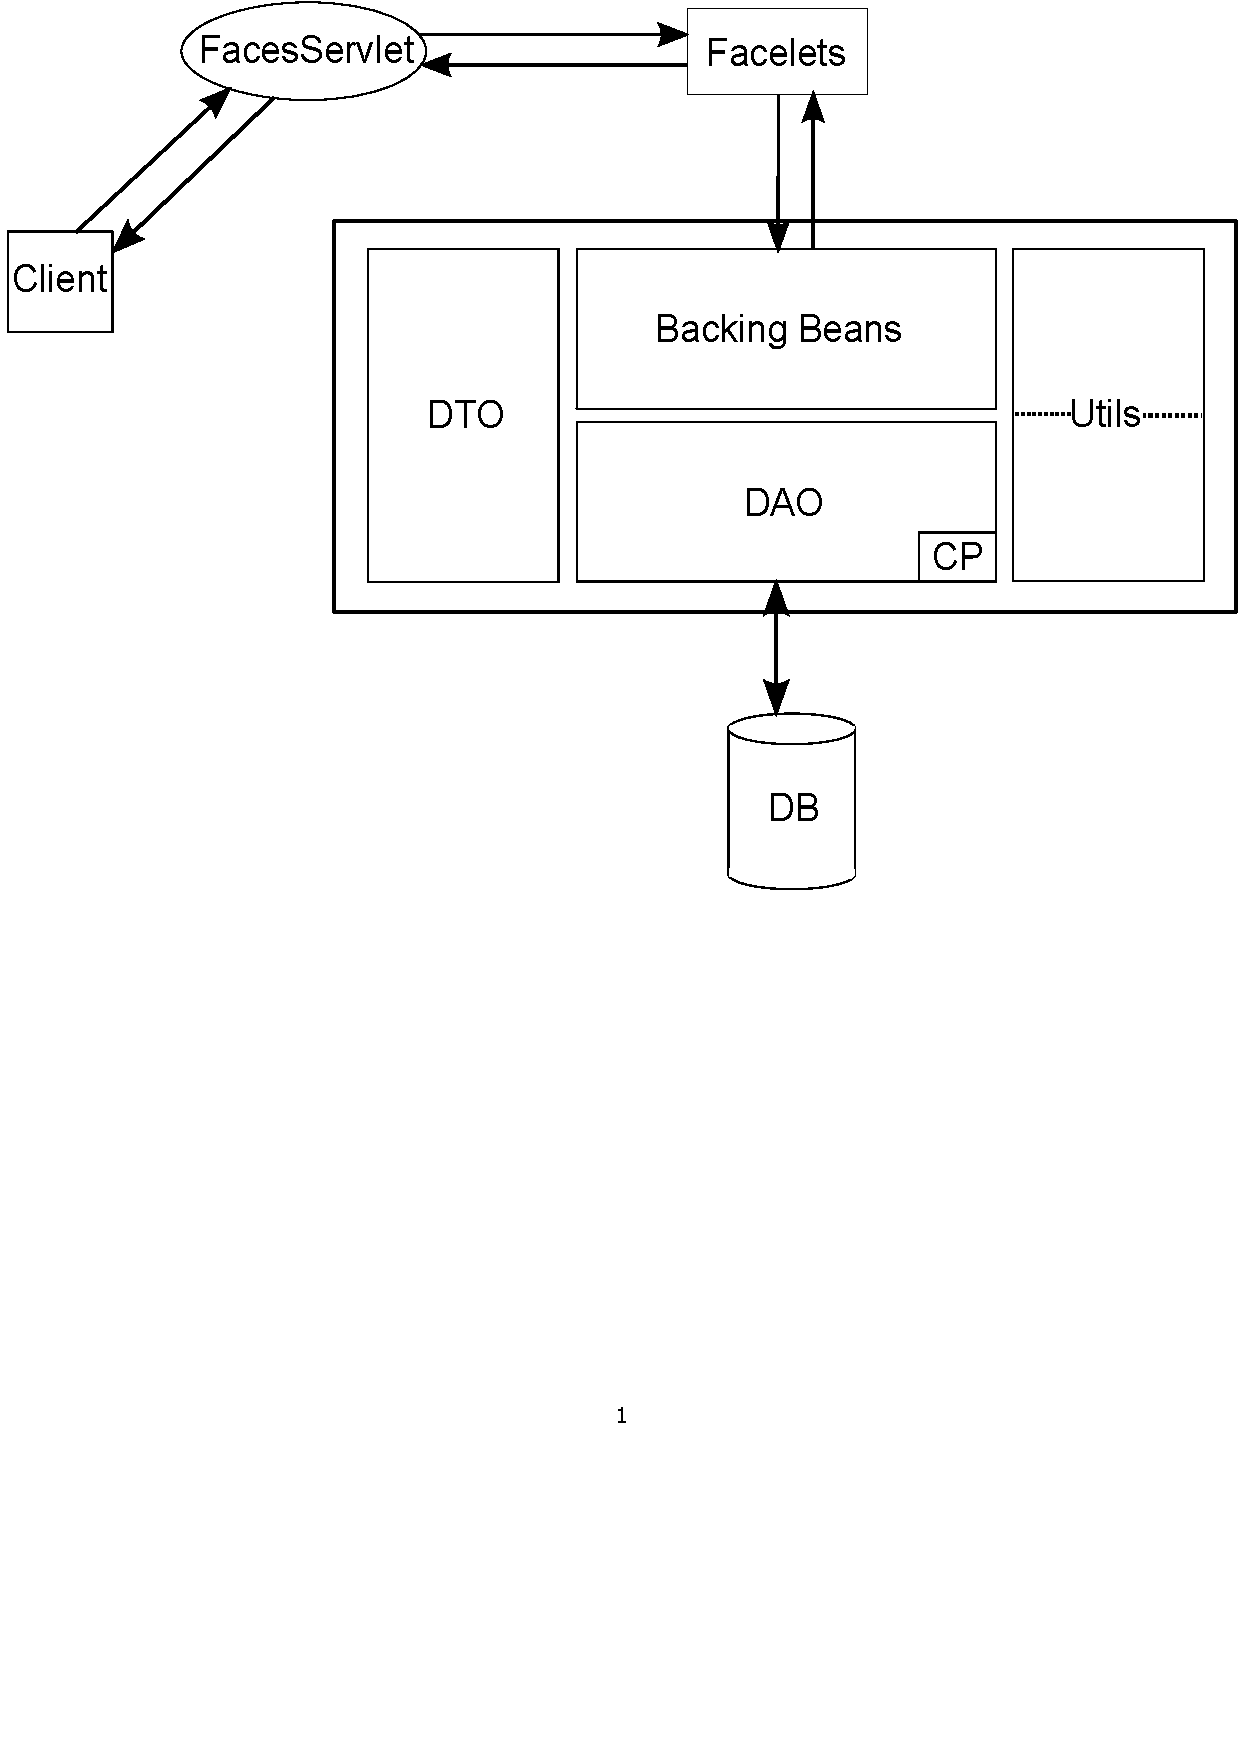
\includegraphics[scale=0.45]{Grafiken/Schichtenarchitektur.pdf}
	\subsection{Faces-Servlet}
	    Das Faces-Servlet fungiert im System als Controller, der eine HTTP-Request abfangt, diese bearbeitet, sowie weiterleitet. Das Faces-Servlet muss in jeder JSF-Applikation konfiguriert sein und wird in der web.xml Datei definiert. 
    \subsection{Facelets}
    	Die View wird durch Facelets repräsentiert. Es stellt den Inhalt dar, der vom Controller übergeben wird. Des Weiteren werden in der View die Benutzerinteraktionen entgegengenommen. 
   	\subsection{Model}
   	Das Model kann in vier Bereiche unterteilt werden. Die Upper Layer, welche die Backing Beans beinhalten, die Lower Layer mit den Data Access Objects (DAOs) und dem Connection Pool (CP), die Data Transfer Objects (DTOs) und den Utils. 
   		\subsubsection{Upper Layer}
   		Die "Upper Layer" besteht aus den Backing Beans. In Diesen ist zum Einen die Geschäftslogik enthalten, zum Anderen werden dort die überlieferten Benutzereingaben der Facelets übergeben, weiterverarbeitet und gespeichert.
    	\subsubsection{Lower Layer}
    	In der "Lower Layer" befinden sich die Data Access Objects und der Connection Pool. Mithilfe des CP greifen die DAOs auf die darunterliegende Database (DB) zu. 
    	\subsubsection{DTO}
    	Die Data Transfer Objects dienen als Schnittstelle zwischen den Backing Beans und den zugehörigen DAOs. Sie bündeln logisch zusammenhängende Daten in einem Objekt, um zeitintensive Fernzugriffe durch einen zu ersetzen.
    	\subsubsection{Utils}
    	Utils fungieren als Hilfs- und Verwalterklasse. Die Utils werden auch wiederum unterteilt, die man entweder den Backing Beans oder den DAOs zuordnen kann. 
    \subsection{Database}
    Die Database (DB) beinhaltet alle relevanten Daten, die für das System benötigt werden. Die DB kapselt die Daten von der Außenwelt ab, somit haben nur die DAOs haben Zugriff auf die DB. 
\section{Design Patterns}
Im Nachfolgendem werden die im System eingesetzten Design Patterns beschrieben.
	\begin{itemize}
		\item Data Transfer Object: Das DTO fassen mehrere Daten in einem Objekt zusammen, damit sie in einem Aufruf übergeben werden. Somit können Datensätze durch die Schichten transportiert werden.
		\item Dependency Injection: 
		\item Object Pooling:
		\item Creational Pattern:
			\begin{itemize}
				\item Factory Pattern:
				\item Singleton:
			\end{itemize}
		\item Singleton:
	\end{itemize}
\section{Fehlerbehandlung}		     


	\newcommand{\class}[1]{\paragraph{Klasse #1:}\ \\ }
	\newcommand{\method}[1]{\textcolor{blue}{#1}}
	\newcommand{\kursiv}[1]{{\it #1}}
	\newcommand{\override}{{\it @Override}\ \\}
	
	\chapter{Klassenbeschreibung und Klassendiagramm}
	In diesem Kapitel werden alle Klassen der Anwendung \textbf{ofCourse} aufgeführt.
	Um eine bessere Übersicht und Strukturierung zu erhalten wird das ganze Projekt in Packages aufgeteilt. Außerdem enthalten folgende Klassen nachfolgende Implementierungen:
	\begin{itemize}
		\item Alle Validator - Klassen: implements Validator
		\item Alle ViewScoped - Klassen: implements Serializable
		\item Alle Exception - Klassen: extends Exception
	\end{itemize}

	\section{Package Action}
		\begin{tiny}
			TF\\
		\end{tiny}\\
	Dieses Package stellt die Businesslogik des Systems \textbf{ofCourse} dar.
	\subsection{Klasse AuthenticateUser}
	\kursiv{ManagedBean, RequestScoped}\\
	Die Klasse ist für die Authentifizierung eines Benutzers im System zuständig.
	\begin{itemize}
		\item \method{public boolean login()}
		\item \method{public User getLoginUser()}
		\item \method{public void setLoginUser(User userToLogIn)}
		\item \method{public SessionUser getSessionUser()}
		\item \method{public void setSessionUser(SessionUser userSession)}
	\end{itemize}
	
	\subsection{Klasse RegisterUser}
	\kursiv{ManagedBean, RequestScoped}\\
	Die Klasse ist für die Registrierung eines Benutzers im System zuständig.
	\begin{itemize}
		\item \method{public boolean registerUser()}
		\item \method{public User getUsertoRegistrate()}
		\item \method{public void setUserToRegistrate(User userToRegistrate)}
		\item \method{public Address getAddress()}
		\item \method{public void setAddress(Address addressToSet)}
		\item \method{public SessionUser getSessionUser()}
		\item \method{public void setSessionUser(SessionUser userSession)}
	\end{itemize}
	
	\subsection{Klasse LostPassword}
	\kursiv{ManagedBean, RequestScoped}\\
	Die Klasse ist für die 'Passwort  vergessen' - Funktion zuständig, d.h. sie ersetzt das alte Passwort eines Benutzers durch ein zufällig generiertes und sendet es an die eingegebene E-Mailadresse.
	\begin{itemize}
		\item \method{public boolean resetPassword()}
		\item \method{public String getEmailAddressToResetPassword()}
		\item \method{public void setEmailAddressToResetPassword(String emailToResetPassword)}
		\item \method{public User getUser()}
		\item \method{public void setUser(User user)}
	\end{itemize}
	
	\subsection{Klasse SearchUser}
	\kursiv{ManagedBean, ViewScoped}\\
	Diese Klasse stellt den Mechanismus zum Suchen von Benutzern zur Verfügung.
	\begin{itemize}
		\item \method{public ArrayList<User> getSearchResult()}
		\item \method{public void setSearchResult(ArrayList<User> searchResult)}
		\item \method{public void search(String searchParam, String searchTerm)}
		\item \method{public String getSearchParam()}
		\item \method{public void setSearchParam(String searchParam)}
		\item \method{public String getSearchTerm()}
		\item \method{public void setSearchTerm(String searchTerm)}
		\item \method{public void sortBySpecificColumn()}
		\item \method{public int getActualPageNumber()}
		\item \method{public void goToSpecificPage()}
		\item \method{public Pagination getPagination()}
		\item \method{public void setPagination(Pagination pagination)}
		\item \method{public SessionUser getSessionUser()}
		\item \method{public void setSessionUser(SessionUser userSession)}
	\end{itemize}
	
	\subsection{Klasse SearchCourse}
	\kursiv{ManagedBean, ViewScoped}\\
	Diese Klasse stellt den Mechanismus zum Suchen von Kursen zur Verfügung. Außerdem wird darin die Einschränkung des angezeigten Kursangebots realisiert.
	\begin{itemize}
		\item \method{public void searchForFreeCourses()}
		\item \method{public void displayCoursesInSpecificPeriod()}
		\item \method{public String getDisplayPeriod()}
		\item \method{public void setDisplayPeriod(String displayPeriod)}
		\item \method{public ArrayList<Course> getSearchResult()}
		\item \method{public void setSearchResult(ArrayList<Course> searchResult)}
		\item \method{public void search(String searchParam, String searchTerm)}
		\item \method{public String getSearchParam()}
		\item \method{public void setSearchParam(String searchParam)}
		\item \method{public String getSearchTerm()}
		\item \method{public void setSearchTerm(String searchTerm)}
		\item \method{public void sortBySpecificColumn()}
		\item \method{public int getActualPageNumber()}
		\item \method{public void goToSpecificPage()}
		\item \method{public Pagination getPagination()}
		\item \method{public void setPagination(Pagination pagination)}
		\item \method{public SessionUser getSessionUser()}
		\item \method{public void setSessionUser(SessionUser userSession)}
	\end{itemize}
	
	\subsection{Klasse UserProfil}
	\kursiv{ManagedBean, ViewScoped}\\
	Diese Klasse ist zuständig für die Anzeige und das Bearbeiten der Benutzerdaten. Des Weiteren realisiert sie die Darstellung der Liste aller vom Benutzer geleiteten Kurse.
	\begin{itemize}
		\item \method{public void editUserdata()}
		\item \method{public void saveUserdata()}
		\item \method{public boolean uploadProfilPic()}
		\item \method{public void setUserInactive()}
		\item \method{public void depositMoneyPerCreditcard()}
		\item \method{public User getUser()}
		\item \method{public void setUser(User userToSet)}
		\item \method{public Address getAddress()}
		\item \method{public void setAddress(Address addressToSet)}
		\item \method{public ArrayList<Course> getManagedCourses()}
		\item \method{public void setManagedCourses(ArrayList<Course> managedCourses)}
		\item \method{public int getActualPageNumber()}
		\item \method{public void goToSpecificPage()}
		\item \method{public Pagination getPagination()}
		\item \method{public void setPagination(Pagination pagination)}
		\item \method{public SessionUser getSessionUser()}
		\item \method{public void setSessionUser(SessionUser userSession)}
	\end{itemize}
	
	\subsection{Klasse CourseDetail}
	\kursiv{ManagedBean, ViewScoped}\\
	Die Klasse ist zuständig für die Anzeige der Kursdetails und das Bearbeiten von Kursen.
	\begin{itemize}
		\item \method{public void editCourse()}
		\item \method{public boolean saveCourse()}
		\item \method{public Course getCourse()}
		\item \method{public void setCourse(Course course)}
		\item \method{public boolean registeredForCourseNews()}
		\item \method{public boolean signUpForCourse() throws CourseRegistrationException}
		\item \method{public boolean signOffForCourse() throws CourseRegistrationException}
		\item \method{public void selectAllCourseUnits()}
		\item \method{public boolean signUpForCourseUnits() throws CourseRegistrationException}
		\item \method{public boolean signOffForCourseUnits() throws CourseRegistrationException}
		\item \method{public ArrayList<CourseUnit> getSelectedCourseUnits()}
		\item \method{public void setSelectedCourseUnits(ArrayList<CourseUnit> selectedCourseUnits)}
		\item \method{public ArrayList<User> getLeadersOfCourse()}
		\item \method{public void setLeadersOfCourse(ArrayList<User> leaders)}
		\item \method{public ArrayList<CourseUnit> getCourseUnitsOfCourse()}
		\item \method{public void setCourseUnitsOfCourse(ArrayList<CourseUnit> courseUnits)}
		\item \method{public String loadParticipientsPage()}
		\item \method{public String loadCreateCourseUnitPage()}
		\item \method{public String loadEditCourseUnitPage()}
		\item \method{public int getActualPageNumber()}
		\item \method{public void goToSpecificPage()}
		\item \method{public Pagination getPagination()}
		\item \method{public void setPagination(Pagination pagination)}
		\item \method{public SessionUser getSessionUser()}
		\item \method{public void setSessionUser(SessionUser userSession)}
	\end{itemize}
	
	\subsection{Klasse CourseUnitManagement}
	\kursiv{ManagedBean, ViewScoped}\\
	Die Klasse ist zuständig für das Anlegen, Bearbeiten und Löschen von Kurseinheiten.
	\begin{itemize}
		 \item \method{public boolean createCourseUnit(boolean isRegular)}
		 \item \method{public void editCourseUnit()}
		 \item \method{public boolean saveCourseUnit(boolean editAllIfRegular)}
		 \item \method{public boolean deleteCourseUnit(boolean deleteAllIfRegular)}
		 \item \method{public boolean addUsersToCourseUnit(ArrayList<User> user)}
		 \item \method{public User getUserToAdd()}
		 \item \method{public void setUserToAdd(User userToAdd)}
		 \item \method{public boolean deleteUserFromCourse()}
		 \item \method{public ArrayList<User> getUserToDelete()}
		 \item \method{public void setUsersToDelete(ArrayList<User> usersToDelete)}
		 \item \method{public boolean getIsRegularCourseUnit()}
		 \item \method{public void setIsRegularCourseUnit(boolean isRegular)}
		 \item \method{public Cycle getCylceOfCourseUnit()}
		 \item \method{public void setCylceOfCourseUnit(Cycle cycle)}
		 \item \method{public CourseUnit getCourseUnit()}
		 \item \method{public void setCourseUnit(CourseUnit courseUnit)}
		 \item \method{public Address getAddress()}
		 \item \method{public void setAddress(Address addressToSet)}
		 \item \method{public ArrayList<User> getParticipientsOfCourseUnit()}
	  	 \item \method{public void setParticipientsOfCourseUnit(ArrayList<User> participients)}
		 \item \method{public int getActualPageNumber()}
		 \item \method{public void goToSpecificPage()}
		 \item \method{public Pagination getPagination()}
		 \item \method{public void setPagination(Pagination pagination)}
		 \item \method{public SessionUser getSessionUser()}
		 \item \method{public void setSessionUser(SessionUser userSession)}
	\end{itemize}
	
	\subsection{Klasse ContactUsers}
	\kursiv{ManagedBean, RequestScoped}\\
	Die Klasse ist zuständig für die Benachrichtigung von Benutzern durch Kursleiter oder Administratoren.
	\begin{itemize}
		\item \method{public boolean sendEMail() throws MailingException}
		\item \method{public Mail getMail()}
	    \item \method{public void setMail(Mail mail)}
		\item \method{public String getSubject()}
		\item \method{public void setSubject(String subject)}
	    \item \method{public String getMessageToSend()}
	    \item \method{public void setMessageToSend(String messageToSend)}
		\item \method{public ArrayList<String> getMailRecipients()}
		\item \method{public void setMailRecipients(ArrayList<String> mailRecipients)}
        \item \method{public SessionUser getSessionUser()}
        \item \method{public void setSessionUser(SessionUser userSession)}
	\end{itemize}
	
	\subsection{Klasse MyCourses}
	\kursiv{ManagedBean, RequestScoped}\\
	Die Klasse ist zuständig für die Anzeige der angemeldeten Kurse eines Benutzers.
	\begin{itemize}
		\item \method{public ArrayList<Course> getRegisteredCourses()}
		\item \method{public void setRegisteredCourses(ArrayList<Course> registeredCourses)}
		\item \method{public String loadCourseDetailsPageOfSelectedCourse()}
		\item \method{public int getActualPageNumber()}
		\item \method{public void goToSpecificPage()}
		\item \method{public Pagination getPagination()}
		\item \method{public void setPagination(Pagination pagination)}
		\item \method{public SessionUser getSessionUser()}
		\item \method{public void setSessionUser(SessionUser userSession)}
	\end{itemize}
	
	\subsection{Klasse CourseManagement}
	\kursiv{ManagedBean, ViewScoped}\\
	Die Klasse ist zuständig für die Verwaltung der Kurse, d.h. für das Anlegen und Löschen von Kursen sowie die Trainerverwaltung.
	\begin{itemize}
		\item \method{public boolean createCourse(Course course)}
		\item \method{public boolean uploadCoursePic()}
		\item \method{public boolean deleteCourse()}
		\item \method{public boolean addCourseLeader(User leader)}
		\item \method{public User getLeaderToAdd()}
		\item \method{public void setLeaderToAdd(User leaderToAdd)}
		\item \method{public boolean removeCourseLeader()}
		\item \method{public boolean removeCourseLeaders()}
		\item \method{public ArrayList<User> getLeadersToDelete()}
		\item \method{public void setLeadersToDelete(ArrayList<User> leadersToDelete)}
		\item \method{public User getCourseLeader()}
		\item \method{public void setCourseLeader()}
		\item \method{public Course getCourse()}
		\item \method{public void setCourse(Course course)}
		\item \method{public Address getAddress()}
		\item \method{public void setAddress(Address address)}
		\item \method{public SessionUser getSessionUser()}
		\item \method{public void setSessionUser(SessionUser userSession)}
	\end{itemize}
	
	\subsection{Klasse AccountManagment}
	\kursiv{ManagedBean, RequestScoped}\\
	Die Klasse ist für die Aktivierung von Benutzeraccounts durch einen Kursleiter oder Administrator zuständig.
	\begin{itemize}
		\item \method{public boolean activateAccounts()}
		\item \method{public ArrayList<User> getUsersToActivate()}
		\item \method{public void setUsersToActivate(ArrayList<User> usersToActivate)}
		\item \method{public ArrayList<User> getSelectedUsers()}
		\item \method{public void setSelectedUsers(ArrayList<User> selectedUsers)}
		\item \method{public int getActualPageNumber()}
		\item \method{public void goToSpecificPage()}
		\item \method{public Pagination getPagination()}
		\item \method{public void setPagination(Pagination pagination)}
		\item \method{public SessionUser getSessionUser()}
		\item \method{public void setSessionUser(SessionUser userSession)}
	\end{itemize}	
	
	\subsection{Klasse UserManagement}
	\kursiv{ManagedBean, ViewScoped}\\
	Die Klasse ist zuständig für die Benutzerverwaltung, d.h. das Anlegen von Benutzern und das Löschen von Benutzern.
	\begin{itemize}
		\item \method{public boolean createUser(User user)}
		\item \method{public boolean uploadProfilPic()}
		\item \method{public boolean deleteUser()}
		\item \method{public User getUser()}
		\item \method{public void setUser(User user)}
		\item \method{public Address getAddress()}
		\item \method{public void setAddress(Address address)}
		\item \method{public SessionUser getSessionUser()}
		\item \method{public void setSessionUser(SessionUser userSession)}
	\end{itemize}
	
	\subsection{Klasse ListParticipents}
	\kursiv{ManagedBean, RequestScoped}\\
	Die Klasse ist zuständig für das Anzeigen der Teilnehmer einer Kurseinheit oder eines Kurses und für die Entfernung einzelner Benutzer aus Kursen oder Kurseinheiten.
	\begin{itemize}
		\item \method{public ArrayList<User> getParticipients()}
		\item \method{public void setParticipients(ArrayList<User> participients)}
		\item \method{public boolean deleteUserFromCourse()}
		\item \method{public ArrayList<User> getUserToDelete()}
		\item \method{public void setUsersToDelete( ArrayList<User> usersToDelete)}
		\item \method{public int getActualPageNumber()}
		\item \method{public void goToSpecificPage()}
		\item \method{public Pagination getPagination()}
		\item \method{public void setPagination(Pagination pagination)}
		\item \method{public SessionUser getSessionUser()}
		\item \method{public void setSessionUser(SessionUser userSession)}
	\end{itemize}
	
	\subsection{Klasse SystemConfiguration}
	\kursiv{ManagedBean, ViewScoped}\\
	Die Klasse ist für Einstellungen bezüglich des Systems zuständig, d.h. das Hochladen einer CSS - Datei, eines Logos, des Festlegen des Überziehungskredits und der Registrierungseinstellungen. Des Weiteren ist sie zuständig für die Weiterleitung zur Benutzer- und Kursverwaltung.
	\begin{itemize}
		\item \method{public void determineAccountActivationType(String accountActivationType)}
		\item \method{public String getAccountActivationType()}
		\item \method{public void setAccountActivationType(String accountActivationType)}
		\item \method{public void determineOverdraftCredit(float overdraftCredit)}
		\item \method{public float getOverdraftCredit()}
		\item \method{public void setOverdraftCredit(float overdraftCredit)}
		\item \method{public boolean uploadCustomStyleCSS()}
		\item \method{public boolean uploadLogo()}
		\item \method{public String loadEditImprintPage()}
		\item \method{public String loadCreateNewUserPage()}
		\item \method{public String loadManageUserPage()}
		\item \method{public String loadCreateNewCoursePage()}
		\item \method{public String loadManageCoursesPage()}
		\item \method{public System getSystem()}
		\item \method{public void setSystem(System system)}
		\item \method{public SessionUser getSessionUser()}
		\item \method{public void setSessionUser(SessionUser userSession)}
	\end{itemize}
	
	\subsection{Klasse PaymentOnline}
	\kursiv{ManagedBean, ViewScoped}\\
	Die Klasse ist zuständig für die Online - Aufladung des Guthabenkontos von Benutzern per Kreditkarte. Die Kreditkartenabwicklung erfolgt über die InfoSun-Bank.
	\begin{itemize}
		\item \method{public boolean depositAmount() throws BankAccountException}
		\item \method{public User getUser()}
		\item \method{public void setUser(User user)}
	    \item \method{public PaymentInformation getPaymentInformation()}
	    \item \method{public void setPaymentInformation(PaymentInformation payInfo)}
		\item \method{public SessionUser getSessionUser()}
		\item \method{public void setSessionUser(SessionUser userSession)}
	\end{itemize}
	
	\subsection{Klasse PaymentOffline}
	\kursiv{ManagedBean, ViewScoped}\\
	Die Klasse ist zuständig für die Offline - Aufladung des Guthabenkontos von Benutzern durch den Administrator und um die Bezahlungseinstellungen zu verwalten.
	\begin{itemize}
		\item \method{public boolean depositAmountOnUserAccount() throws BankAccountException}
		\item \method{public User getUser()}
		\item \method{public void setUser(User user)}
		\item \method{public int getAmountToDeposit()}
		\item \method{public void setAmountToDeposit(float amountToDeposit)}
		\item \method{public SessionUser getSessionUser()}
		\item \method{public void setSessionUser(SessionUser userSession)}
	\end{itemize}
	
	\subsection{Klasse IncomeStatistics}
	\kursiv{ManagedBean, RequestScoped}\\
	Die Klasse ist für die Generierung und Darstellung der Einnahmestatistiken zuständig.
	\begin{itemize}
	    \item \method{public void displayStatistic(String displayParam)}
		\item \method{public String getDisplayParam()}
		\item \method{public void setDisplayParam(String displayParam)}
		\item \method{public int getActualPageNumber()}
		\item \method{public void goToSpecificPage()}
		\item \method{public Pagination getPagination()}
		\item \method{public void setPagination(Pagination pagination)}
		\item \method{public SessionUser getSessionUser()}
		\item \method{public void setSessionUser(SessionUser userSession)}
	\end{itemize}
	
	\subsection{Klasse EditImprint}
	\kursiv{ManagedBean, ViewScoped}\\
	Die Klasse ist für die Darstellung und Bearbeitung des Impressums verantwortlich.
	\begin{itemize}
		\item \method{public void editImprint(String imprint)}
		\item \method{public String getImprint()}
		\item \method{public void setImprint(String imprint)}
		\item \method{public SessionUser getSessionUser()}
		\item \method{public void setSessionUser(SessionUser userSession)}
	\end{itemize}
	
	\subsection{Klasse Header}
	\kursiv{ManagedBean, RequestScoped}\\
	Diese Klasse ist zuständig für das Laden der Anmeldeseite, das Abmelden und der Auswahl der Anzeigesprache.
	\begin{itemize}
		\item \method{public String login()}
		\item \method{public boolean logout()}
		\item \method{public String getChoosenLanguage()}
		\item \method{public void setChoosenLanguage(String choosenLanguage)}
		\item \method{public SessionUser getSessionUser()}
		\item \method{public void setSessionUser(SessionUser userSession)}
	\end{itemize}
	
	\subsection{Klasse Footer}
	\kursiv{ManagedBean, RequestScoped}\\
	Diese Klasse ist zuständig für das Laden der AGB, der Hilfe und der Impressumsseite.
	\begin{itemize}
		\item \method{public String loadImprintPage()}
		\item \method{public String loadAGBPage()}
		\item \method{public String loadHelpPage()}
	\end{itemize}
	
	\subsection{Klasse Scheduler}
	\kursiv{ManagedBean, RequestScoped}\\
	Diese Klasse ist zuständig für die Generierung und Darstellung des persönlichen Terminplaners des Benutzers.
	\begin{itemize}
		\item \method{public void displayScheduler(ArrayList<CourseUnit> bookedCourseUnits)}
		\item \method{public void displayNextWeek()}
		\item \method{public void displayPreviousWeek()}
		\item \method{public SessionUser getSessionUser()}
		\item \method{public void setSessionUser(SessionUser userSession)}
	\end{itemize}
	
	\subsection{Klasse SessionUser}
	\kursiv{ManagedBean, SessionScoped}\\
	Die Klasse speichert Informationen über die Session eines Benutzers. Gespeichert werden die ID des Benutzers, dessen Benutzerrolle, der aktuelle Status des Benutzers und die gewählte Sprache.
	\begin{itemize}
		\item \method{public int getUserID()}
		\item \method{public void setUserID(int userID)}
		\item \method{public int getUserStatus()}
		\item \method{public void setUserStatus(int userStatus)}
		\item \method{public String getUserRole()}
		\item \method{public void setUserRole(String userRole)}
		\item \method{public String getLanguage()}
		\item \method{public void setLanguage(String language)}
	\end{itemize}
	
	\subsection{Klasse Mail}
	\kursiv{ManagedBean, ApplicationScoped}\\
	Die Klasse ist für die E-Mailbenachrichtigung der Benutzer zuständig. Sie ist sowohl für die automatisch gesendeten E-Mails, wie unter anderem die Verifizierung oder Accountaktivierungsbestätigung, als auch für die von Kursleitern gesendeten Mails zuständig.
	\begin{itemize}
		\item \method{public boolean sendVerificationMail(int UserID) throws MailingException}
		\item \method{public boolean sendConfirmaitionMail(int UserID) throws MailingException}
		\item \method{public boolean sendMail(String subject, String message, ArrayList<String> mailRecipients) throws MailingException}
		\item \method{public SmtpServer getSmtpServer()}
		\item \method{public void setSmtpServer(SmtpServer smtpServer)}
	\end{itemize}
	
	\section{Package Model}
	\begin{tiny}
		SeSc \\
	\end{tiny}\\
	Das Pakte Model enthält die Klassen für Aufzählungstypen. Die privaten Attribute können durch die jeweiligen \glqq getter\grqq- \ und \glqq setter\grqq- \ Methoden aufgerufen und gesetzt werden.
	\subsection{Klasse SmtpServer}
	Die Klasse enthält die Zugangsdaten des E-Mail Servers.
	\begin{itemize}
		\item \method {public String getHostaddr()}
		\item \method {public String getPassword()}
		\item \method {public int getPort()}
		\item \method {public String getUsername()}
		\item \method {public boolean isAuthentificated()}
		\item \method {public boolean isTls()}
		\item \method {public void setAuthentificated(Boolean authentificated)}
		\item \method {public void setHostaddr(String hostaddr)}
		\item \method {public void setPassword(String password)}
		\item \method {public void setPort(int port)}
		\item \method {public void setTls(Boolean tls)}
		\item \method {public void setUsername(String username)}
	
	\end{itemize}
	
	\subsection{Klasse Pagination}
	Die Klasse steuert die Anzeige von Listen der Kurse, Benutzer und Benutzereinheiten um Skalierbarkeit zu bewahren.
	\begin{itemize}
		\item \method {public int getItemsPerPage()}
		\item \method {public int getShownPageNum()}
		\item \method {public String getSortColumn()}
		\item \method {public boolean isSortAsc()}
		\item \method {public void setItemsPerPage(int itemsPerPage)}
		\item \method {public void setSortColumn(String sortColumn)}
		\item \method {public void setShownPageNum(int shownPageNum)}
		\item \method {public void setSortAsc(boolean sortAsc)}
	\end{itemize}
	
	\subsection{Klasse Course}
	\begin{itemize}
		\item \method {public String getTitle()}
		\item \method {public String getDiscription()}
		\item \method {public CourseUnit getNextCourseUnit()}
		\item \method {public Date getStartdate()}
		\item \method {public Date getEnddate()}
		\item \method {public int getMaxUsers()}
		\item \method {public ArrayList<CourseUnit> getCourseUnits()}
		\item \method {public ArrayList<User> getCoursAdmins()}
		\item \method {public ArrayList<User> getUsers()}
		\item \method {public ArrayList<User> getUsersToInform()}
		\item \method {public void setTitle(String title)}
		\item \method {public void setDiscription(String discription)}
		\item \method {public void setNextCourseUnit(CourseUnit nextCourseUnit)}
		\item \method {public void setStartdate(Date startDate)}
		\item \method {public void setEnddate(Date endDate)}
		\item \method {public void setMaxUsers(int maxUsers)}
		\item \method {public void setCourseUnits(ArrayList<CourseUnit> courseUnits) }
		\item \method {public void setCourseAdmins(ArrayList<User> coursAdmins)}
		\item \method {public void setUsers(ArrayList<User> users)}
		\item \method {public void setUsersToInform(ArrayList<User> usersToInform)}  
	\end{itemize}
	
	
	\subsection{Klasse CourseUnit}
	\begin{itemize}
		\item \method {public String getTitle()}
		\item \method {public String getDiscription()}
		\item \method {public Date getStarttime()}
		\item \method {public Date getEndtime()}
		\item \method {public Address getAddress()}
		\item \method {public float getPrice()}
		\item \method {public int getMaxUsers()}
		\item \method {public int getMinUsers()}
		\item \method {public User getCourseAdmin()}
		\item \method {public ArrayList<User> getUsers()}
		\item \method {public void setTitle(String title)}
		\item \method {public void setDiscription(String discription)}
		\item \method {public void setStarttime(Date startingTime)}
		\item \method {public void setEndtime(Date endTime)}
		\item \method {public void setAddress(Address address)}
		\item \method {public void setPrice(float price)}
		\item \method {public void setMaxUsers(int maxUsers)}
		\item \method {public void setMinUsers(int minUsers)}
		\item \method {public void setCourseAdmin(User courseAdmin)}
		\item \method {public void setUsers(ArrayList<User> users)} 
		\end{itemize}
	
	
	\subsection{Klasse User}
	Diese Klasse stellt alle Benutzer des Systems dar. Je nach Status des Benutzers(Administrator, Kursleiter und Benutzer) sind unterschiedliche Attribute ausgefüllt.
	\begin{itemize}
		\item \method {public Address getAddress()}
		\item \method {public boolean equals(Object other)}
		\item \method {public String getEmail()}
		\item \method {public String getFristname()}
		\item \method {public String getLastname()}
		\item \method {public String getUsernname()}
		\item \method {public String getPassword()}
		\item \method {public Date getDateOfBirth()}
		\item \method {public UserRole getUserRole()}
		\item \method {public int getUserID()}
		\item \method {public int hashCode()}
		\item \method {public void setAddress(Address address)}
		\item \method {public void setEmail(String email)}
		\item \method {public void setFirstname(String firstname)}
		\item \method {public void setLastname(String lastname)}
		\item \method {public void setPassword(String password)}
		\item \method {public void setUserRole(UserRole role)}
		\item \method {public void setUserId(int id)}
		\item \method {public void setUsername(String username)}
		\item \method {public void setDateOfBirth(Date dateOfBirth)}
	\end{itemize}
	\subsection{Enumeration UserRole}
	Es werden nun die verschiedenen Benutzerrollen beschrieben.
	\begin{itemize}
		\item {REGISTERED\_USER}
		\item {COURSE\_LEADER}
		\item {SYSTEM\_ADMINISTRATOR}
	\end{itemize}
	
	\subsection{Enumeration UserStatus}
	Es werden nun die verschiedenen Statuszustände eines Benutzers beschrieben.
	\begin{itemize}
		\item {ANONYMOUS}
		\item {NOT\_ACTIVATED}
		\item {REGISTERED}
		\item {INACTIVE}
	\end{itemize}

	
	\subsection{Klasse Address}
	Diese Klasse verwaltet die Adressenangaben der Kurseinheiten und Benutzer.
	\begin{itemize}
		\item \method {public boolean equals(Object other)}
		\item \method {public String getCountry()}
		\item \method {public String getTown()}
		\item \method {public String getStreet()}
		\item \method {public String getRoom()}
		\item \method {public int getHouseNumber()}
		\item \method {public int getZipCode()}
		\item \method {public void setCountry(String country)}
		\item \method {public void setTown(String town)}
		\item \method {public void setStreet(String street)}
		\item \method {public void setRoom(String room)}
		\item \method {public void setHouseNumber(int houseNumber)}
		\item \method {public void setZipCode(int zipCode)}
		
	\end{itemize}
	
	\subsection{Klasse PaymentInformation}
	Diese Klasse stellt die Kreditkarteninformationen, Bankdaten und den Einzahlungsbetrag
	dar.
	\begin{itemize}
		\item \method{public String getAccountNumber()}
		\item \method{ public void setAccountNumber(String accountNumber)}
		\item \method{public int getAmount()}
		\item \method{ public void setAmount(int amount)}
		\item \method{public String getCcHolder()}
		\item \method{ public void setCcHolder(String ccHolder)}
		\item \method{ public String getCcNumber()}
		\item \method{ public void setCcNumber(String ccNumber)}
		\item \method{ public Date getCcValidFrom()}
		\item \method{ public void setCcValidFrom(Date ccValidFrom)}
		\item \method{ public Date getCcValidTo()}
		\item \method{ public void setCcValidTo(Date ccValidTo)}
		\item \method{ public int getCvc()}
		\item \method{ public void setCvc(int cvc)}
		
	\end{itemize}
	
	\subsection{Klasse System}
	In dieser Klasse werden die editierbaren Eigenschaften des Systems gespeichert.
	\begin{itemize}
		\item \method {public boolean equals(Object other)}
		\item \method {public String getCSS()}
		\item \method {public String getImpressum()}
		\item \method {public String getLogo()}
		\item \method {public String getTitle()}
		\item \method {public void setCss(String css)}
		\item \method {public void setImpressum (String impressum)}
		\item \method {public void setLogo(String logo)}
		\item \method {public void setTitle(String title)}
	\end{itemize}
	
	\section{Package Services}
	\begin{tiny}
		TF
	\end{tiny}
    \subsection{Klasse HttpsHelper}
    Dies ist eine Hilfsklasse für Https-Verbindungen.
    \begin{itemize}
    	\item \method{public static void setup()}
    \end{itemize}
    
    \subsection{Klasse TransferAction}
    Diese Klasse übermittelt die Zahlungsdaten an die Bank und liefert eine Zahlungsbestätigung
    zurück.
	    \begin{itemize}
	    	\item \method{public static boolean executeBankTransaktion(PaymentInformation payInfo)}
	    \end{itemize}
    
	\section{Package Interfaces}
	\begin{tiny}
		TF\\
	\end{tiny}\\
	Dieses Package stellt Interfaces zur Verfügung, welche die DAO - Klassen implementieren müssen damit gegebenenfalls  ein Wechsel der Datenbank einfach möglich ist.
	    \class{UserInteraction}
		Dieses Interface gibt vor, welche Methoden für Datenbankanfragen für das Erhalten bzw. das Schreiben von Benutzerdaten vorhanden sein müssen.
		\begin{itemize}
			\item \method{public boolean createUser(User user, Address address)}
			\item \method{public ArrayList<User> getUsers(Pagination pagination)}
			\item \method{public ArrayList<User> getUsers(Pagination pagination, String searchString)}
			\item \method{public ArrayList<User> getUsersOrdered(Pagination pagination, String searchString, String orderParam)}
			\item \method{public User getUser(int userID)}
			\item \method{public int getUserID(String username)}
			\item \method{public boolean updateUser(User user, Address address)}
			\item \method{public boolean deleteUser(int userID)}
			\item \method{public ArrayList<Course> getCoursesLeadedBy(int userID, Pagination pagination)}
		\end{itemize}
		
		\class{CourseInteraction}
		Dieses Interface gibt vor, welche Methoden für Datenbankanfragen für das Erhalten bzw. das Schreiben von Kursdaten vorhanden sein müssen.
		\begin{itemize}
			\item \method{public boolean createCourse(Course course, Address address)}
			\item \method{public ArrayList<Course> getCourses(Pagination pagination)}
			\item \method{public ArrayList<Course> getCourses(Pagination pagination, String searchString)}
			\item \method{public ArrayList<Course> getCoursesOrdered(Pagination pagination, String searchString, String orderParam)}
			\item \method{public ArrayList<User> getLeaders(int courseID)}
			\item \method{public Course getCourse(int courseID)}
			\item \method{public boolean updateCourse(Course course, Address address)}
			\item \method{public boolean deleteCourse(int courseID)}
			\item \method{public boolean addUserToCourse(int userID)}
			\item \method{public boolean removeUserFromCourse(int userID)}
			\item \method{public boolean addLeaderToCourse(int userID)}
			\item \method{public boolean removeLeaderFromCourse(int userID)}
		\end{itemize}
		
		\class{CourseUnitInteraction}
			Dieses Interface gibt vor, welche Methoden für Datenbankanfragen für das Erhalten bzw. das Schreiben von Kurseinheitsdaten vorhanden sein müssen.
		\begin{itemize}
			\item \method{public boolean createCourseUnit(CourseUnit courseUnit, Address address)}
			\item \method{public CourseUnit getCourseUnit(int courseUnitID)}
			\item \method{public ArrayList<CourseUnit> getCourseUnitsFromCourse(int courseID, Pagination pagination)}
			\item \method{public boolean updateCourseUnit(CourseUnit courseUnit, Address address)}
			\item \method{public boolean deleteCourseUnit(int courseUnitID)}
			\item \method{public boolean addUserToCourseUnit(int userID)}
			\item \method{public boolean removeUserFromCourseUnit(int userID)}
		\end{itemize}
		
		\class{StatisticsInteraction}
			Dieses Interface gibt vor, welche Methoden für Datenbankanfragen für das Erhalten von Statistikdaten oder das Schreiben dieser in die Datenbank vorhanden sein müssen.
			\begin{itemize}
				\item \method{public HashMap<Date, Float> getIncomePerDay(Date actualDate)}
				\item \method{public HashMap<Date, Float> getIncomePerWeek(Date actualDate)}
				\item \method{public HashMap<User, Float> getIncomePerLeader(Pagination pagination)}
				\item \method{public HashMap<Course, Float> getIncomePerCourse(Pagination pagination)}
			\end{itemize}
		
	\section{Package Database}
	\begin{tiny}
		TF
	\end{tiny}
	\subsection{Package DatabaseGeneral}
	
		\class{SetupAdmin}
		Diese Klasse ist zuständig für das Erstellen des ersten Systemadministrators.
		\begin{itemize}
			\item \method{public boolean createInitialAdmin()}
			\item \method{public boolean createDefaultImprint()}
		\end{itemize}
	
		\class{DatabaseTableCreator}
		Diese Klasse ist zuständig für das Erstellen der Tabellen in der Datenbank, falls diese noch nicht existieren.
		\begin{itemize}
			\item \method{public static boolean buildUpDatabase() throws InvalidDatabaseTransferException}
		\end{itemize}
	
		\class{DatabaseTableDetroyer}
		Diese Klasse ist zuständig für das Löschen der Tabellen in der Datenbank, falls diese existieren.
		\begin{itemize}
			\item \method{public static boolean destroyDatabaseTables() throws InvalidDatabaseTransferException}
		\end{itemize}
	
	\subsection{Package DAO}
		\class{UserDAO}
		Diese Klasse stellt Datenbankanfragen zur Verfügung um Benutzerdaten zu erhalten oder in die
		Datenbank zu schreiben.\\
		Sämtliche Methoden können die \kursiv{InvalidDatabaseTransferException} werfen.
		\begin{itemize}
			\item \method{public boolean createUser(User user, Address address)}
			\item \method{public ArrayList<User> getUsers(Pagination pagination)}
			\item \method{public ArrayList<User> getUsers(Pagination pagination, String searchString)}
			\item \method{public ArrayList<User> getUsersOrdered(Pagination pagination, String searchString, String orderParam)}
			\item \method{public User getUser(int userID)}
			\item \method{public int getUserID(String username)}
			\item \method{public boolean updateUser(User user, Address address)}
			\item \method{public boolean deleteUser(int userID)}
			\item \method{public ArrayList<Course> getCoursesLeadedBy(int userID, Pagination pagination)}
			\end{itemize}
		
		\class{CourseDAO}
		Diese Klasse stellt Datenbankanfragen zur Verfügung um Kursdaten zu erhalten oder in die Datenbank
		zu schreiben.\\
		Sämtliche Methoden können die \kursiv{InvalidDatabaseTransferException} werfen.
		\begin{itemize}
			\item \method{public boolean createCourse(Course course, Address address)}
			\item \method{public ArrayList<Course> getCourses(Pagination pagination)}
			\item \method{public ArrayList<Course> getCourses(Pagination pagination, String searchString)}
			\item \method{public ArrayList<Course> getCoursesOrdered(Pagination pagination, String searchString, String orderParam)}
			\item \method{public ArrayList<User> getLeaders(int courseID)}
			\item \method{public Course getCourse(int courseID)}
			\item \method{public boolean updateCourse(Course course, Address address)}
			\item \method{public boolean deleteCourse(int courseID)}
			\item \method{public boolean addUserToCourse(int userID)}
			\item \method{public boolean removeUserFromCourse(int userID)}
			\item \method{public boolean addLeaderToCourse(int userID)}
			\item \method{public boolean removeLeaderFromCourse(int userID)}
		\end{itemize}
		
		\class{CourseUnitDAO}
		Diese Klasse stellt Datenbankanfragen zur Verfügung um Kurseinheitsdaten zu erhalten oder in die Datenbank zu schreiben.\\
		Sämtliche Methoden können die \kursiv{InvalidDatabaseTransferException} werfen.
		\begin{itemize}
			\item \method{public boolean createCourseUnit(CourseUnit courseUnit, Address address)}
			\item \method{public CourseUnit getCourseUnit(int courseUnitID)}
			\item \method{public ArrayList<CourseUnit> getCourseUnitsFromCourse(int courseID, Pagination pagination)}
			\item \method{public boolean updateCourseUnit(CourseUnit courseUnit, Address address)}
			\item \method{public boolean deleteCourseUnit(int courseUnitID)}
			\item \method{public boolean addUserToCourseUnit(int userID)}
			\item \method{public boolean removeUserFromCourseUnit(int userID)}
		\end{itemize}
		
		\class{StatisticDAO}
		Diese Klasse stellt Datenbankanfragen zur Verfügung um Statistikdaten zu erhalten oder in die Datenbank
		zu schreiben.\\
		Sämtliche Methoden können die \kursiv{InvalidDatabaseTransferException} werfen.
		\begin{itemize}
			\item \method{public HashMap<Date, Float> getIncomePerDay(Date actualDate)}
			\item \method{public HashMap<Date, Float> getIncomePerWeek(Date actualDate)}
			\item \method{public HashMap<User, Float> getIncomePerLeader(Pagination pagination)}
			\item \method{public HashMap<Course, Float> getIncomePerCourse(Pagination pagination)}
		\end{itemize}
	
	\section{Package System}
	\begin{tiny}
		TF
	\end{tiny}
	\subsection{Klasse CheckPhase}
	Die Klasse ist zuständig für die Überprüfung, ob der jeweilige Benutzer die Berechtigung besitzt, auf die angeforderte Seite zu gelangen.\\
	Die Klasse implementiert das Interface PhaseListener.
	\begin{itemize}
		\item \method{public PhaseId getPhaseId()}
		\item \override
		\method{public void beforePhase(PhaseEvent arg0)}
		\item \override
		\method{public void afterPhase(PhaseEvent event)}	
	\end{itemize}
	
	\subsection{Klasse Maintenance}
	Die Klasse ist zuständig den Wartungsthread, der dafür sorgt, dass Kurse sechs Monate nach ihrem Enddatum automatisch aus dem System gelöscht werden.\\
	Die Klasse implementiert das Interface Runnable.
	\begin{itemize}
		\item \method{public boolean isMaintenaceStopped()}
		\item \method{public synchronized void shutDown()}
		\item \method{public static Maintenance getInstance()}
		\item \override
		\method{public void run()}
	\end{itemize}
	
	\subsection{Klasse LaunchSystem}
	\kursiv{ManagedBean, ApplicationScoped}\\
	Die Klasse ist zuständig für das Starten des System. Sie startet den Maintenance - Thread, lädt Properties und stellt die Datenbankverbindung her.
	\begin{itemize}
		\item \kursiv{@PostConstruct}\\
		\method{public void startSystem()}
		\item \kursiv{@PreDestroy}\\
		\method{public void shutdownMaintenance()}
	\end{itemize}
	
	\subsection{Klasse DatabaseConnectionManager}
	Die Klasse ist zuständig für das Aufbauen der Verbindungen zur Datenbank. Des Weiteren
	speichert und verwaltet sie die Datenbankverbindungen. 
	\begin{itemize}
		\item \method{public synchronized Connection getConnection()}
		\item \method{public synchronized void releaseConnection()}
		\item \method{public static DatabaseConnectionManager getInstance()}
		\item \method{public void shutDown()}
	\end{itemize}
	
	
	\section{Package Util}
	\begin{tiny}
		TF
	\end{tiny}
	\subsection{Klasse PasswordHash}
	Diese Klasse ist zuständig für das Hashen der Passwörter.
	\begin{itemize}
		\item \method{public static String hash(String password, int salt)}
	\end{itemize}
	
	\subsection{Klasse LanguageManagager}
	Diese Klasse ist zuständig für die angezeigte Systemsprache. In ihr werden die unterstützten Sprachen verwaltet und sie ist zuständig für das Auslesen der Anzeigetexte aus der Properties - Datei der gewählten Sprache.
	\begin{itemize}
		\item \method{public static LanguageManager getInstance()}
		\item \method{public LinkedHashMap<String, Object> getSupportedLanguages()}
		\item \method{public String getProperty(String key)}
		\item \method{public void switchLanguage(String language)}
	\end{itemize}
	
	\subsection{Klasse PropertyManager}
	Die Klasse ist zuständig für das Auslesen der Property - Datei, welche die Daten für die Systemkonfiguration, also die Daten für die Datenbankverbindung und den E-Mail - Service enthält.
	\begin{itemize}
		\item \method{public static PropertyManager getInstance()}
		\item \method{public String getProperty(String key)}
		\item \method{public String setProperty(String key)}
	\end{itemize}
	
	\subsection{Klasse IDGenerator}
	Die Klasse ist zuständig für das Generieren einer im System eindeutigen Identifikationsnummer für einen Benutzer, einen Kurs oder eine Kurseinheit.
	\begin{itemize}
		\item \method{public static int generateUserID()}
		\item \method{public static int generateCourseID()}
		\item \method{public static int generateCourseUnitID(int CourseID)}
	\end{itemize}
	
	\subsection{Klasse RandomSaltGenerator}
	Die Klasse ist zuständig für das Generieren eines zufälligen Salt, welcher für das Hashen des Benutzerpassworts benötigt wird.
	\begin{itemize}
		\item \method{public static int generateRandomSalt()}
	\end{itemize} 
	
	\subsection{Klasse EncodingFilter}
	Diese Klasse implementiert die Filter - Methoden um UTF-8 Encoding zu
	ermöglichen und somit Probleme bei der Zeichendarstellung zu verhindern.
	\begin{itemize}
		\item \override
		\method{public void destroy()}
		\item \override
		\method{public void doFilter(ServletRequest request, ServletResponse response,
			FilterChain chain)}
		\item \override
		\method{public void init(FilterConfig filterConfig)}
	\end{itemize}
	
	\section{Package Exception}
	\begin{tiny}
		SeSc
	\end{tiny}
	\subsection{Klasse CustomExceptionHandler}
	Diese Klasse ist zuständig für die Weiterleitung zu Fehlerseiten, falls ein Fehler aufgetreten
	ist. \\
	Die Klasse CustomExceptionHandler erbt aus ExceptionHandlerWrapper.
		\begin{itemize}
			\item \override
			\method{public ExceptionHandler getWrapped()}
		\end{itemize}
		
	\subsection{Klasse CustomExceptionHandlerFactory}
	Diese Klasse ist zuständig für das  Initialisieren des CustomExceptionHandler-Objekts, welches die auftretenden Fehler behandeln soll.\\
	Die Klasse CustomExceptionHandlerFactory erbt aus ExceptionHandlerFactory.
	\begin{itemize}
		\item \override
		\method{public ExceptionHandler getExceptionHandler()}
	\end{itemize}
	
	\subsection{BankAccountException}
	Diese Klasse behandelt Exceptions im Zusammenhang mit der Bankverbindung.
	
	\subsection{MailingException}
	Diese Klasse behandelt Exceptions im Zusammenhang mit der E-Mailversendung.
	
	\subsection{CourseRegistrationException}
    Dies sind Fehler, welche beim An- oder Abmelden zu Kursen/Kurseinheiten auftreten können. 
	
	\subsection{InvalidDatabaseTransferException}
	Diese Klasse behandelt SQL-Exceptions und  TimeOut - Exceptions im Zusammenhang mit der Datenbankverbindungen.
	
	\section{Package CustomValidator}
	\begin{tiny}
		TF\\
	\end{tiny}\\
	Dieser Abschnitt beschäftigt sich mit den benötigten Validatoren, die notwendig sind, um die Eingaben des Benutzers zu überprüfen und gegebenenfalls Fehlermeldungen zu generieren.\\
	Alle Klassen dieses Packages implementieren das Interface Validator.
	
	\subsection{Klasse UserNameValidator}
	Der Validator überprüft, ob der eingegebene Benutzername schon im System vergeben ist.
	\begin{itemize}
		\item \override
		\method{public void validate()}
	\end{itemize}
	
	\subsection{Klasse EMailValidator}
	Der Validator überprüft, ob die Eingabe ein gültiges E-Mail-Format besitzt und ob die eingegebene E-Mailadresse bereits im System existiert.
	\begin{itemize}
		\item \override
		\method{public void validate()}
	\end{itemize}
	
	\subsection{Klasse PasswordValidator}
	Dieser Validator überprüft, ob das eingegebene Passwort gewisse Sicherheitsanforderungen bezüglich Länge und Zeichenwahl erfüllt. Vorgesehene Anforderungen an das Passwort sind mindestens 8 Zeichen, mindestens ein Sonderzeichen, mindestens eine Ziffer, Verwendung von Groß- und Kleinbuchstaben. Außerdem dürfen im Passwort keine Umlaute sowie kein \grq ß\grq \ vorkommen.
	\begin{itemize}
		\item \override
		\method{public void validate()}
	\end{itemize}
	
	\subsection{Klasse ConfirmPasswordValidator}
	Dieser Validator überprüft zwei Passwörter auf ihre Übereinstimmung.
	\begin{itemize}
		\item \override
		\method{public void validate()}
	\end{itemize}
	
	\subsection{Klasse DateOfBirthValidator}
	Der Validator überprüft, ob das eingegebene Datum eingegebene Datum in der Zukunft liegt oder ob es mehr als 150 Jahre zurückliegt.
	\begin{itemize}
		\item \override
		\method{public void validate()}
	\end{itemize}
	
	\subsection{Klasse UserImageValidator}
	Dieser Validator überprüft eine Bilddatei auf die richtige Dateiendung .jpg. Zusätzlich wird überprüft, ob
	die maximale Dateigröße und die maximal zugelassene Auflösung für ein Profilbild eines Benutzers eingehalten wird.
	\begin{itemize}
		\item \override
		\method{public void validate()}
	\end{itemize}
	
	\subsection{Klasse DateValidator}
	Der Validator überprüft Datumseingaben.
	\begin{itemize}
		\item \override
		\method{public void validate()}
	\end{itemize}
	
	\subsection{Klasse CreditCardValidator}
	Der Validator überprüft, ob eine Kreditkartenummer gültig ist.
	\begin{itemize}
		\item \override
		\method{public void validate()}
	\end{itemize}
	
	\subsection{Klasse CVCValidator}
	Dieser Validator überprüft eine CVC Nummer auf ihre Gültigkeit.
	\begin{itemize}
		\item \override
		\method{public void validate()}
	\end{itemize}
	
	\subsection{Klasse InputTextValidator}
	Überprüft den eingegebenen Text auf korrekte Zeichenkodierung.
	\begin{itemize}
		\item \override
		\method{public void validate()}
	\end{itemize}
	
	\subsection{Klasse OfflineTransactionValidator}
	Dieser Validator überprüft, ob bei einer Offline-Aufladung des Guthabenkontos eines Benutzers der eingegebene Name und die eingegebenen Benutzeridentifikationsnummer auch zum selben Benutzer gehören.
	\begin{itemize}
		\item \override
		\method{public void validate()}
	\end{itemize}
	
	\subsection{Klasse PriceValidator}
	Der Validator überprüft, ob der eingegebene Preis das korrekte Format hat, dass heißt, ob die Zahl nicht-negativ ist und zwei Nachkommastellen besitzt.
	\begin{itemize}
		\item \override
		\method{public void validate()}
	\end{itemize}
	
	\subsection{Klasse ImageValidator}
	Dieser Validator überprüft eine Bilddatei auf die richtige Dateiendung .jpg. Zusätzlich wird überprüft, ob
	die maximale Dateigröße und die maximal zugelassene Auflösung für ein Bild(Logo oder Kursbild) eingehalten wird.
	\begin{itemize}
		\item \override
		\method{public void validate()}
	\end{itemize}
	
	\subsection{Klasse CustomStyleCSSValidator}
	Der Validator überprüft, ob die Datei den Namen 'customStyle' besitzt und ob es sich um den Dateityp mit der Endung .css handelt.
	\begin{itemize}
		\item \override
		\method{public void validate()}
	\end{itemize}
		
	\section{Verwendete Libraries}
	\begin{tiny}
		TF\\
	\end{tiny}\\
	In dem System zusätzlich verwendete Libraries:
	\begin{itemize}
		\item Commons Fileupload: Library für das Hochladen von Dateien.
		\item JavaMail: Library für das Versenden von E-Mails.
		\item JFreeChart: Library für die Erstellung von Diagrammen.
		\item Log4J: Library für das Loggen von Meldungen.
	\end{itemize}

	\section{Klassendiagramm}
	\begin{tiny}
		Diagramm: SeSc und TF\ \ Layout: SeSc\\
	\end{tiny}\\
	Um sich dieses Diagramm genauer ansehen zu können, muss es mit einem PDF-Reader
	geöffnet werden, der eine Zoom-Funktion besitzt.
	
	\begin{center}
		\includegraphics[width=1.0\linewidth]{Grafiken/OfCourseumlcd}
		Abbildung: UML-Klassendiagramm des ofCourse-Systems
	\end{center}



\chapter{Facelets}

	Dieses Kapitel enthält alle benötigten  Facelets. Jedes Facelet wird in unterschiedliche  Bereiche aufgeteilt:
	\begin{itemize}
		\item \textbf{Beschreibung} beinhaltet die Funktionen des Facelets.
		\item \textbf{Links} enthält die Seiten, auf welche weitergeleitet wird.
		\item \textbf{Buttons} listet die sich auf der Seite befindlichen Buttons mit deren hinterlegten Methoden auf.
		\item \textbf{Inputs} enthält eine Liste aller Eingabefelder auf der Seite.
		\item \textbf{Outputs} enthält eine Liste aller Ausgabefelder auf der Seite.
		\item \textbf{Backing Bean} gibt das mit dem Facelet verbundene Bean an.
	\end{itemize}
	
	\section{Templates}
		Kathi, Ricky
	
		\paragraph{layout.xhtml}
		
		\paragraph{header.xhtml}
		
		\paragraph{footer.xhtml}
	
	\section{Facelets}
	
		\subsection{open}
			
			\subsubsection{common}
			
				\paragraph{index.xhtml}
					RS\\
					\begin{itemize}
						\item \textbf{Beschreibung:} Dieses Facelet stellt die Startseite des Systems dar.
						\item \textbf{Links:}
							\begin{itemize}
								\item Gesamtes Kursangebot, listCourses.xhtml
							\end{itemize}
						\item \textbf{Buttons:} -
						\item \textbf{Inputs:} -
						\item \textbf{Outputs:}
							\begin{itemize}
								\item Logo der Website
							\end{itemize}
						\item \textbf{BackingBean:}
					\end{itemize}
				
				\paragraph{authenticate.xhtml}
				KH\\
				\begin{itemize}
					\item \textbf{Beschreibung:}
					Auf dieser Seite kann man sich im System anmelden, ein neues Benutzerkonto generieren oder ein neues Passwort anfordern.
					\item \textbf{Links:} -
					\item \textbf{Buttons:}
						\begin{itemize}
							\item Registrieren: Durch Drücken dieses Buttons wird der neue Benutzer mit den eingegebenen Daten im System gespeichert und es wird eine Bestätigungsmail mit dem Verifizierungslink an die angegebene E-Mail-Adresse verschickt, sofern alle Daten korrekt eingegeben wurden.
							\item Anmelden: Durch Drücken dieses Buttons wird der registrierte Benutzer im System angemeldet und auf die Seite 'Meine Kurse' weitergeleitet, sofern Benutzername und Passwort korrekt eingegeben wurden.
							\item Neues Passwort anfordern: Durch Drücken dieses Buttons wird an die angegebene E-Mail-Adresse ein automatisch generiertes Passwort geschickt, sofern die Adresse im System existiert.
						\end{itemize}
					\item \textbf{Inputs:}
						\begin{itemize}
							\item Anrede (Registrierung): Hier wählt der Benutzer die Anrede 'Herr' oder 'Frau' aus.
							\item Vorname (Registrierung): Hier trägt der Benutzer seinen Vornamen ein.
							\item Name (Registrierung): Hier gibt der Benutzer seinen Namen ein.
							\item Benutzername (Registrierung): Hier gibt der Benutzer einen Benutzernamen ein.
							\item Passwort (Registrierung): Hier trägt der Benutzer ein Passwort ein.
							\item Passwort bestätigen (Registrierung): Hier gibt der Benutzer das gleiche Passwort erneut ein zur Bestätigung.
							\item Geburtstag (Registrierung): Hier gibt der Benutzer sein Geburtsdatum ein.
							\item Straße/Hausnummer (Registrierung): Hier gibt der Benutzer seine Straße und seine Hausnummer ein.
							\item Stadt (Registrierung): Hier trägt der Benutzer seine Stadt ein.
							\item Postleitzahl (Registrierung): Hier trägt der Benutzer seine Postleitzahl ein.
							\item Land (Registrierung): Hier trägt der Benutzer sein Heimatland ein.
							\item E-Mail-Adresse (Registrierung): Hier gibt der Benutzer seine E-Mail-Adresse ein.
							\item AGBs bestätigen (Registrierung): Durch Setzten des Häkchens bestätigt der Benutzer die AGBs. 
							\item Benutzername (Anmeldung): Der Benutzer gibt seinen Benutzernamen ein, mit dem er sich registriert hat.
							\item Passwort (Anmeldung): Der Benutzer gibt sein Passwort ein, mit dem er sich registriert hat.
							\item E-Mail-Adresse (Passwort vergessen): Der Benutzer gibt seine im System bereits gespeicherte E-Mailadresse ein.
						\end{itemize}
					\item \textbf{Outputs:} 
						\begin{itemize}
							\item Vorname Fehlermeldung (Registrierung): Ausgabe der Fehlermeldungen zu den Validatoren des Eingabefeldes.
							\item Name Fehlermeldung (Registrierung): Ausgabe der Fehlermeldungen zu den Validatoren des Eingabefeldes.
							\item Benutzername Fehlermeldung (Registrierung): Ausgabe der Fehlermeldungen zu den Validatoren des Eingabefeldes.
							\item Passwort Fehlermeldung (Registrierung): Ausgabe der Fehlermeldungen zu den Validatoren des Eingabefeldes.
							\item Passwort bestätigen Fehlermeldung (Registrierung): Ausgabe der Fehlermeldungen zu den Validatoren des Eingabefeldes.
							\item Geburtstag Fehlermeldung (Registrierung): Ausgabe der Fehlermeldungen zu den Validatoren des Eingabefeldes.
							\item Straße/Hausnummer Fehlermeldung (Registrierung): Ausgabe der Fehlermeldungen zu den Validatoren des Eingabefeldes.
							\item Stadt Fehlermeldung (Registrierung): Ausgabe der Fehlermeldungen zu den Validatoren des Eingabefeldes.
							\item Postleitzahl Fehlermeldung (Registrierung): Ausgabe der Fehlermeldungen zu den Validatoren des Eingabefeldes.
							\item Land Fehlermeldung (Registrierung): Ausgabe der Fehlermeldungen zu den Validatoren des Eingabefeldes.
							\item E-Mail-Adresse Fehlermeldung (Registrierung): Ausgabe der Fehlermeldungen zu den Validatoren des Eingabefeldes.
							\item AGBs bestätigen Fehlermeldung (Registrierung): Ausgabe der Fehlermeldungen zu den Validatoren des Eingabefeldes.
							\item Benutzername Fehlermeldung (Anmeldung): Ausgabe der Fehlermeldungen zu den Validatoren des Eingabefeldes.
							\item Passwort Fehlermeldung (Anmeldung): Ausgabe der Fehlermeldungen zu den Validatoren des Eingabefeldes.
							\item E-Mail-Adresse Fehlermeldung (Passwort vergessen): Ausgabe der Fehlermeldungen zu den Validatoren des Eingabefeldes.
						\end{itemize}
					\item \textbf{BackingBean:} authenticate.java
				\end{itemize}
				
				\paragraph{imprint.xhtml}
					KH\\
					\begin{itemize}
						\item \textbf{Beschreibung:} Auf dieser Seite kann das Impressum angesehen werden.
						\item \textbf{Links:} -
						\item \textbf{Buttons:} -
						\item \textbf{Inputs:} -
						\item \textbf{Outputs:} 
							\begin{itemize}
								\item	Anzeige des Impressums, welches vom Administrator festgelegt wurde.
							\end{itemize}
						\item \textbf{BackingBean:} -
					\end{itemize}
				
				\paragraph{agb.xhtml}
					RS\\
					\begin{itemize}
						\item \textbf{Beschreibung:} Dieses Facelet dient der Anzeige der Allgemeinen Geschäftsbedingungen.
						\item \textbf{Links:} -
						\item \textbf{Buttons:} -
						\item \textbf{Inputs:} -
						\item \textbf{Outputs:}
							\begin{itemize}
								\item von Betreibern festgelegte Allgemeine Geschäftsbedingungen.
							\end{itemize}
						\item \textbf{BackingBean:} -
					\end{itemize}
				\paragraph{navigation.xhtml}
					RS\\
					\begin{itemize}
						\item \textbf{Beschreibung:} Hier kann, abhängig von der Benutzerrolle, durch die Seite navigiert werden.
						\item \textbf{Links:}
							\begin{itemize}
								\item Suche: Navigiert zur Kurse durchsuchen Seite.
								\item Sprache Deutsch: Ändert die angezeigte Sprache zu Deutsch.
								\item Sprache Englisch: Ändert die angezeigte Sprache zu Englisch.
								\item Profil (Benutzer): Navigiert zum eigenen Profil.
								\item Meine Kurse (Benutzer): Navigiert zur Anzeige der eigenen Kurse.
								\item Terminplaner (Benutzer): Navigiert zum persönlichen Terminplaner.
							\end{itemize}
						\item \textbf{Buttons:}
							\begin{itemize}
								\item Logout (Benutzer, wenn eingeloggt): Loggt den aktuellen eingeloggten Benutzer aus.
								\item Anmelden (Anonym): Navigiert zur Registrierungs- und Anmeldeseite.
							\end{itemize}
						\item \textbf{Inputs:} -
						\item \textbf{Outputs:}
							\begin{itemize}
								\item persönliche Loginbenachrichtigung (Benutzer, wenn eingeloggt).
								\item Logo: Zeigt verkleinertes, vom Administrator definiertes Logo der Website.
							\end{itemize}
						\item \textbf{BackingBean:}
					\end{itemize}
		
			\subsubsection{courses}
				
				\paragraph{listCourses.xhtml}
					RS\\
					\begin{itemize}
						\item \textbf{Beschreibung:} Hier können alle Kurse angezeigt und durchsucht werden.
						\item \textbf{Links:} -
						\item \textbf{Buttons:}
							\begin{itemize}
								\item Anzeigen: Zeigt die Angebote im ausgewählten Zeitraum an.
								\item Suchen: Durchsucht die Website nach dem eingegebenen Suchbegriff mittels gewählten Suchobjekt.
							\end{itemize}
						\item \textbf{Inputs:}
							\begin{itemize}
								\item Angebotszeitraum: Ermöglicht eine genauere Anzeige des Kursangebots, entweder Tagesangebot, Wochenangebot oder das gesamte Angebot. Die detaillierteren Suchoptionen sind nur für registrierte Benutzer verfügbar.
								\item Suchobjekt (abhängig von Benutzerrolle): Ermöglicht eine genauere Suche, beispielsweise nach Kursen, Kursleitern oder Kurs-ID.
							\end{itemize}
						\item \textbf{Outputs:}
							\begin{itemize}
								\item Tabelle mit Ergebnissen der Suche.
								\item Schaltfläche um zwischen Ergebnissen zu Blättern.
							\end{itemize}
						\item \textbf{BackingBean:}
					\end{itemize}
				
				\paragraph{courseDetails.xhtml}
					RS\\
					\begin{itemize}
						\item \textbf{Beschreibung:} Detailanzeige eines einzelnen Kurses.
						\item \textbf{Links:} -
						\item \textbf{Buttons:}
							\begin{itemize}
								\item Anmelden (Benutzer, noch nicht angemeldet): Meldet den Benutzer zum Kurs an.
								\item Abmelden (Benutzer, wenn angemeldet): Meldet den Benutzer vom Kurs ab.
								\item Teilnehmer anzeigen (Kursleiter): Zeigt die zum Kurs angemeldeten Benutzer an.
								\item Alle auswählen (Benutzer, zum Kurs angemeldet): Wählt alle Kurseinheiten des Kurses aus.
								\item Speichern (Benutzer, zum Kurs angemeldet): Speichert alle ausgewählten Kurseinheiten und meldet den Nutzer dazu an.
								\item Bearbeiten (Administrator, noch nicht im Bearbeitungsmodus): Ermöglicht die Bearbeitung der einzelnen Kursdetails.
								\item Speichern (Administrator, im Bearbeitungsmodus): Speichert alle vorgenommenen Kursänderungen.
								\item Hinzufügen (Administrator): Fügt einen Kursleiter zum Kurs hinzu.
								\item Kurseinheit anlegen (Kursleiter): Erstellt eine neue Kurseinheit zum Kurs.
								\item Kurseinheit bearbeiten (Kursleiter): Ermöglicht die Bearbeitung einer einzelnen Kurseinheit.
								\item Kurs löschen (Administrator): Löscht den Kurs.
							\end{itemize}
						\item \textbf{Inputs:}
							\begin{itemize}
								\item Kursnews erhalten: Trägt Benutzer bei Anmeldung zum Kurs in die Kursnews ein.
								\item Kurseinheit auswählen: Wählt Kurseinheit aus, zu der sich der Nutzer anmelden möchte.
								\item Kursleiter auswählen (Administrator): Wählt Kursleiter aus, welcher gelöscht werden soll.
								\item Kursleiter Name (Administrator): Eingabefeld für den Namen eines neuen Kursleiters.
								\item Kursleiter E-Mail (Administrator): Eingabefeld für die E-Mail Adresse eines neuen Kursleiters.
								\item Kursbeschreibung (Administrator): Eingabefeld für die Kursbeschreibung.
								\item Minimale Teilnehmerzahl (Administrator): Eingabefeld für die minimale Teilnehmerzahl des Kurses.
								\item Startdatum (Administrator): Eingabefeld für das Startdatum des Kurses.
								\item Enddatum (Administrator): Eingabefeld für das Enddatum des Kurses.
							\end{itemize}
						\item \textbf{Outputs:}
							\begin{itemize}
								\item Tabelle Kursleiter: Tabelle mit den Kontaktinformationen der/des Kursleiters.
								\item Tabelle Kurseinheiten: Tabelle mit allen Kurseinheiten des Kurses und zugehörigen Informationen wie Ort, Preis oder Datum.
								\item Kurs-ID: Zeigt die zum Kurs zugehörige ID an.
								\item Fehlermeldung zu den einzelnen Eingabefeldern, bei falscher Eingabe.
							\end{itemize}
						\item \textbf{BackingBean:}
					\end{itemize}
		
		\subsection{users}
		
			\subsubsection{registeredUser}
				
				\paragraph{myCourses.xhtml}
					KH\\
					\begin{itemize}
						\item \textbf{Beschreibung:} Auf dieser Seite werden alle Kurse angezeigt, in die der Teilnehmer eingetragen ist.
						\item \textbf{Links:}
							\begin{itemize}
								\item Kurstitel: Über die Kurstitel gelangt der Benutzer auf die jeweilige Kursdetailseite.
							\end{itemize}
						\item \textbf{Buttons:}
						\item \textbf{Inputs:} -
						\item \textbf{Outputs:}
							\begin{itemize}
								\item Tabelle Auflistung aller Kurse: Hier werden dem Benutzer alle seine angemeldeten Kurse angezeigt.
							\end{itemize}
						\item \textbf{BackingBean:} myCourses.java
					\end{itemize}
				
				\paragraph{profile.xhtml}
					KH\\
					\begin{itemize}
						\item \textbf{Beschreibung:} Auf dieser Seite werden die persönlichen Daten und der Kontostand des Benutzers angezeigt. Der Benutzer kann die Daten ändern und sein Konto aufladen. Der Kursleiter kann hier den Benutzer aktivieren, und der Administrator den Benutzer löschen.
						\item \textbf{Links:} -
						\item \textbf{Buttons:}
							\begin{itemize}
								\item Bearbeiten: Nach Klicken auf diesen Button können die persönlichen Daten geändert werden. Der Button trägt nun die Aufschrift 'Speichern' und ist mit dessen dazugehöriger Methode hinterlegt.
								\item Speichern: Durch Drücken dieses Buttons werden die vorgenommenen Änderungen gespeichert, sofern alle Daten korrekt eingegeben wurden. Bei Änderung der E-Mail-Adresse wird außerdem eine Bestätigungsmail mit einem Verifizierungslink verschickt. Bei erfolgreicher Speicherung erscheint der Button 'Bearbeiten' anstelle des Button 'Speichern'.
								\item Durchsuchen: Durch Drücken dieses Buttons kann das eigene Dateiverzeichnis nach einem Bild durchsucht und hochgeladen werden.
								\item Konto aufladen: Durch Klicken dieses Buttons wird der Benutzer auf die Seite 'Kontoaufladung' weitergeleitet.
								\item Benutzer löschen: Durch Drücken dieses Buttons entfernt der Administrator diesen Benutzer aus dem System.
								\item Benutzer aktivieren: Durch diesen Button kann der Benutzer je nach Einstellung der Accountaktivierung vom Kursleiter oder vom Administrator aktiviert werden.
							\end{itemize}
						\item \textbf{Inputs:}
							\begin{itemize}
								\item Vorname: Hier kann der Benutzer seinen Vornamen ändern.
								\item Name: Hier kann der Benutzer seinen Namen ändern.
								\item Geburtstag: Hier kann der Benutzer sein Geburtsdatum ändern.
								\item Straße/Hausnummer: Hier kann der Benutzer seine Straße und Hausnummer ändern.
								\item Stadt: Hier kann der Benutzer seine Stadt ändern.
								\item Postleitzahl: Hier kann der Benutzer seine Postleitzahl ändern.
								\item Land: Hier kann der Benutzer seine Land ändern.
								\item E-Mail-Adresse: Hier kann der Benutzer seine E-Mail-Adresse ändern.
								\item Benutzername: Hier kann der Benutzer seinen Benutzernamen ändern.
								\item Passwort: Hier kann der Benutzer sein Passwort ändern.
								\item Passwort bestätigen: Hier muss der Benutzer sein geändertes Passwort bestätigen.
								\item Benutzerrolle: Hier kann der Administrator die Benutzerrolle eines Nutzers ändern.
								\item Profilbild: Hier kann der Benutzer sein Profilbild ändern.
							\end{itemize}
						\item \textbf{Outputs:}
							\begin{itemize}
								\item Benutzer-ID: Ausgabe der automatisch generierten ID.
								\item Vorname Fehlermeldung: Ausgabe der Fehlermeldungen zu den Validatoren des Eingabefeldes.
								\item Name Fehlermeldung: Ausgabe der Fehlermeldungen zu den Validatoren des Eingabefeldes.
								\item Geburtstag Fehlermeldung: Ausgabe der Fehlermeldungen zu den Validatoren des Eingabefeldes.
								\item Straße/Hausnummer Fehlermeldung: Ausgabe der Fehlermeldungen zu den Validatoren des Eingabefeldes.
								\item Stadt Fehlermeldung: Ausgabe der Fehlermeldungen zu den Validatoren des Eingabefeldes.
								\item Postleitzahl Fehlermeldung: Ausgabe der Fehlermeldungen zu den Validatoren des Eingabefeldes.
								\item Land Fehlermeldung: Ausgabe der Fehlermeldungen zu den Validatoren des Eingabefeldes.
								\item E-Mail-Adresse Fehlermeldung: Ausgabe der Fehlermeldungen zu den Validatoren des Eingabefeldes.
								\item Benutzername Fehlermeldung: Ausgabe der Fehlermeldungen zu den Validatoren des Eingabefeldes.
								\item Passwort Fehlermeldung: Ausgabe der Fehlermeldungen zu den Validatoren des Eingabefeldes.
								\item Passwort bestätigen Fehlermeldung: Ausgabe der Fehlermeldungen zu den Validatoren des Eingabefeldes.
								\item Profilbild Fehlermeldung: Ausgabe der Fehlermeldungen zu den Validatoren des Eingabefeldes.
								\item Kontostand: Ausgabe des aktuellen Kontostandes.
								\item Tabelle Auflistung der Trainingskurse: Hier werden dem Kursleiter alle Kurse aufgelistet, die er leitet.
							\end{itemize}
						\item \textbf{BackingBean:} profile.java
					\end{itemize}
				
				\paragraph{buyCredits.xhtml}
					RS\\
					\begin{itemize}
						\item \textbf{Beschreibung:} Hier kann der Nutzer mittels Kreditkarte seinen systeminternen Kontostand erhöhen.
						\item \textbf{Links:} -
						\item \textbf{Buttons:}
							\begin{itemize}
								\item Konto aufladen: Führt die Kontoaufladung aus.
							\end{itemize}
						\item \textbf{Inputs:}
							\begin{itemize}
								\item Benutzer-ID: Benutzer-ID des Nutzers zur Kontoaufladung.
								\item Benutzername: Benutzername des Nutzers zur Kontoaufladung.
								\item Nachname: Nachname des Nutzers zur Kontoaufladung.
								\item Vorname: Vorname des Nutzers zur Kontoaufladung.
								\item Kreditinstitut: Name des Kreditinstitutes des Nutzers zur Kontoaufladung.
								\item Kreditkartennummer: Nummer der Kreditkarte des Nutzers zur Kontoaufladung.
								\item Betrag: Geldbetrag, welcher auf das systeminterne Konto des Nutzers gebucht werden soll.
							\end{itemize}
						\item \textbf{Outputs:}
							\begin{itemize}
								\item Fehlermeldung zu den einzelnen Eingabefeldern, bei falscher Eingabe.
							\end{itemize}
						\item \textbf{BackingBean:}
					\end{itemize}
				
				\paragraph{scheduler.xhtml}
					RS\\
					\begin{itemize}
						\item \textbf{Beschreibung:} Persönlicher Terminplaner mit anstehenden Kursen.
						\item \textbf{Links:}
							\begin{itemize}
								\item Wochenansicht vorwärts: Zeigt die Termine der nächsten Woche an.
								\item Wochenansicht rückwärts: Zeigt die Termine der letzten Woche an.
							\end{itemize}
						\item \textbf{Buttons:} -
						\item \textbf{Inputs:} -
						\item \textbf{Outputs:}
							\begin{itemize}
								\item Wochentabelle: Zeigt von Montag bis Sonntag alle belegten Kurseinheiten an. Orientiert sich am klassischen Stundenplan, also mit stündlicher Ansicht.
							\end{itemize}
						\item \textbf{BackingBean:}
					\end{itemize}
				
				\paragraph{leaderProfile.xhtml}
					KH\\
					\begin{itemize}
						\item \textbf{Beschreibung:} Auf dieser Seite werden die Daten des Kursleiters, mit Ausnahme von sensiblen Daten wie Passwort oder Kontostand, und die von ihm geleiteten Kurse angezeigt.
						\item \textbf{Links:} -
						\item \textbf{Buttons:} -
						\item \textbf{Inputs:} -
						\item \textbf{Outputs:} 
							\begin{itemize}
								\item Tabelle Auflistung Kursleiterdaten: Hier werden die Daten des Kursleiters und die von ihm geleiteten Kurse angezeigt.
							\end{itemize}
						\item \textbf{BackingBean:} leaderProfile.java
					\end{itemize}
				
				\paragraph{listParticipants.xhtml}
					KH\\
					\begin{itemize}
						\item \textbf{Beschreibung:} Hier kann der registrierte Benutzer die Teilnehmer eines Kurses mit Benutzername und Profilbild ansehen. Dem Kursleiter werden zusätzlich die E-Mail-Adresse und die Information über den Erhalt von Kursnews angezeigt. Außerdem kann er einen Teilnehmer aus dem Kurs entfernen.
						\item \textbf{Links:} -
						\item \textbf{Buttons:}
							\begin{itemize}
								\item Löschen: Durch Drücken dieses Buttons kann der Kursleiter den entsprechenden Benutzer aus dem Kurs entfernen.
							\end{itemize}
						\item \textbf{Inputs:}
							 \begin{itemize}
							 	\item Entfernen: Durch Setzen des Häkchens wählt der Kursleiter diesen Benutzer aus, um ihn anschließend über den Button 'Löschen' zu entfernen.
							 \end{itemize}
						\item \textbf{Outputs:} -
						\item \textbf{BackingBean:} listParticipants.java
					\end{itemize}
			
			\subsubsection{courseLeader}
			
				\paragraph{editCourseUnit.xhtml}
					KH\\
					\begin{itemize}
						\item \textbf{Beschreibung:} Auf dieser Seite können Kursleiter beziehungsweise Administrator Kurseinheiten anlegen und bearbeiten, oder Kursteilnehmer hinzufügen und entfernen
						\item \textbf{Links:} -
						\item \textbf{Buttons:}
							\begin{itemize}
								\item Bearbeiten (Kurseinheit): Nach Klicken auf diesen Button können die Daten der Kurseinheit geändert beziehungsweise eingetragen werden. Der Button trägt nun die Aufschrift 'Speichern' und ist mit dessen dazugehöriger Methode hinterlegt.
								\item Speichern (Kurseinheit): Durch Drücken dieses Buttons werden die vorgenommenen Änderungen gespeichert, sofern alle Daten korrekt eingegeben wurden. Bei erfolgreicher Speicherung erscheint der Button 'Bearbeiten' anstelle des Button 'Speichern'.
								\item Löschen (Kurseinheit): Durch Drücken des Button 'Löschen' wird die Kurseinheit entfernt.
								\item Löschen (Teilnehmer): Durch Drücken dieses Buttons wird der markierte Teilnehmer aus der Kurseinheit entfernt.
								\item Hinzufügen (Teilnehmer): Durch Drücken dieses Buttons wird der angegebene Teilnehmer zu dieser Kurseinheit hinzugefügt, sofern der Benutzername im System existiert und die Daten korrekt eingegeben wurden.
							\end{itemize}
						\item \textbf{Inputs:}
							\begin{itemize}
								\item Termin: Hier gibt der Kursleiter den Termin der Kurseinheit ein.
								\item Straße/ Hausnummer: Hier gibt der Kursleiter Straße und Hausnummer ein.
								\item Postleitzahl: Hier gibt der Kursleiter die entsprechende Postleitzahl ein.
								\item Stadt: Hier gibt der Kursleiter die Stadt ein, in der die Kurseinheit stattfindet.
								\item Raum: Hier gibt der Kursleiter den Raum ein, in dem die Kurseinheit stattfindet.
								\item Beschreibung: Hier gibt der Kursleiter die Beschreibung der Kurseinheit ein.
								\item Preis: Hier gibt der Kursleiter den Preis der Kurseinheit ein.
								\item Kursleiter: Hier wird der Leiter des Kurses angezeigt.
								\item Mindestteilnehmerzahl: Hier gibt der Kursleiter die minimale Teilnehmerzahl der Kurseinheit an.
								\item Maximale Teilnehmerzahl: Hier gibt der Kursleiter die maximale Teilnehmerzahl der Kurseinheit an.
								\item Teilnehmer markieren: Hier kann der Kursleiter einen Hacken setzen, um den Teilnehmer für das anschließende Löschen zu markieren.
								\item Benutzer-ID: Hier gibt der Kursleiter die Benutzer-ID des Teilnehmers an, welchen er zu der Kurseinheit hinzufügen will.
								\item Name (Teilnehmer): Hier gibt der Kursleiter den entsprechenden Namen des Teilnehmers an, welchen er zu der Kurseinheit hinzufügen will.
								\item Vorname (Teilnehmer): Hier gibt der Kursleiter den entsprechenden Vornamen des Teilnehmers an, welchen er zu der Kurseinheit hinzufügen will.
							\end{itemize}
						\item \textbf{Outputs:}
							\begin{itemize}
								\item Termin (Fehlermeldung): Ausgabe der Fehlermeldungen zu den Validatoren des Eingabefeldes.
								\item Straße/ Hausnummer (Fehlermeldung): Ausgabe der Fehlermeldungen zu den Validatoren des Eingabefeldes.
								\item Postleitzahl (Fehlermeldung): Ausgabe der Fehlermeldungen zu den Validatoren des Eingabefeldes.
								\item Stadt (Fehlermeldung): Ausgabe der Fehlermeldungen zu den Validatoren des Eingabefeldes.
								\item Raum (Fehlermeldung): Ausgabe der Fehlermeldungen zu den Validatoren des Eingabefeldes.
								\item Beschreibung (Fehlermeldung): Ausgabe der Fehlermeldungen zu den Validatoren des Eingabefeldes.
								\item Preis (Fehlermeldung): Ausgabe der Fehlermeldungen zu den Validatoren des Eingabefeldes.
								\item Kursleiter (Fehlermeldung): Ausgabe der Fehlermeldungen zu den Validatoren des Eingabefeldes.
								\item Mindestteilnehmerzahl (Fehlermeldung): Ausgabe der Fehlermeldungen zu den Validatoren des Eingabefeldes.
								\item Maximale Teilnehmerzahl (Fehlermeldung): Ausgabe der Fehlermeldungen zu den Validatoren des Eingabefeldes.
								\item Status: Hier wird ausgegeben, wie viele Teilnehmer bereits in der Kurseinheit eingetragen sind.
								\item Benutzer-ID (Fehlermeldung): Ausgabe der Fehlermeldungen zu den Validatoren des Eingabefeldes.
								\item Name (Teilnehmer (Fehlermeldung)): Ausgabe der Fehlermeldungen zu den Validatoren des Eingabefeldes.
								\item Vorname (Teilnehmer (Fehlermeldung)): Ausgabe der Fehlermeldungen zu den Validatoren des Eingabefeldes.
							\end{itemize}
						\item \textbf{BackingBean:} editCourseUnit.java
					\end{itemize}
				
				\paragraph{listUsers.xhtml}
					KH\\
					\begin{itemize}
						\item \textbf{Beschreibung:} Hier werden alle im System registrierten Benutzer angezeigt. Einzelne Benutzer können nach verschiedenen Kriterien gefiltert werden oder der Administrator kann den Account von Benutzern aktiveren. 
						\item \textbf{Links:} -
						\item \textbf{Buttons:}
							\begin{itemize}
								\item Suchen: Durch Drücken dieses Buttons werden die Benutzer nach den eingegebenen Kriterien durchsucht und in der Liste angezeigt.
								\item Benutzer aktivieren: Durch Klicken dieses Buttons wird der Account des markierten Benutzers aktiviert.
							\end{itemize}
						\item \textbf{Inputs:}
							\begin{itemize}
								\item Kriterienauswahl: Hier kann der Kursleiter auswählen, ob er nach 'Benutzer-ID', 'Benutzername', 'Name' 'Benutzerrolle' oder 'nicht aktiviert' suchen will.
								\item Suchbegriff: Hier gibt der Kursleiter den entsprechenden Suchbegriff ein.
								\item Benutzer aktivieren: Der Administrator kann durch Setzen des Häkchens Benutzer auswählen, um diese anschließend zu aktivieren.
							\end{itemize}
						\item \textbf{Outputs:}
							\begin{itemize}
								\item Tabelle Auflistung Benutzerdaten: Hier werden ausgewählte Daten aller im System registrierten Benutzer angezeigt.
								\item Suchbegriff (Fehlermeldung): Ausgabe der Fehlermeldungen zu den Validatoren des Eingabefeldes.
							\end{itemize}
						\item \textbf{BackingBean:}
					\end{itemize}
			
			\subsubsection{systemAdministrator}
			
				\paragraph{adminManagement.xhtml}
					RS\\
					\begin{itemize}
						\item \textbf{Beschreibung:} Dieses Facelet stellt die zentrale Systemverwaltung für den Administrator dar. Hier kann er Kurse und Benutzer jeweils anlegen und verwalten, das Konto eines Nutzers aufladen, zu den Statistiken gelangen, den Überziehungskredit für Nutzer festlegen und das System optisch anpassen.
						\item \textbf{Links:} -
						\item \textbf{Buttons:}
							\begin{itemize}
								\item Benutzer verwalten: Navigiert zu Benutzer verwalten Seite
								\item Benutzer anlegen: Navigiert zu Benutzer anlegen Seite
								\item Kurse verwalten: Navigiert zu Kurse verwalten Seite
								\item Kurs anlegen: Navigiert zu Kurs anlegen Seite
								\item Aktivierungsmodalität speichern: Speichert die ausgewählte Art der Benutzeraktivierung
								\item Guthaben aufladen: Erhöht den Kontostand eines bestimmten Benutzer um die eingegebene Summe 
								\item Überziehungswert speichern: Speichert den Wert der möglichen Kontoüberziehung
								\item Statistiken anzeigen: Navigiert zur Anwendungsstatistik Seite
								\item Logo durchsuchen: Öffnet ein Fenster um das Logo der Website vom Computer auszuwählen
								\item Logo speichern: Speichert das benutzerdefinierte Logo für die Website
								\item Oberfläche CSS durchsuchen: Öffnet ein Fenster um die benutzerdefinierte CSS-Datei vom Computer auszuwählen
								\item Oberfläche CSS speichern: Speichert die benutzerdefinierte CSS-Datei
								\item Impressum bearbeiten: Navigiert zur Impressum bearbeiten Seite
							\end{itemize}
						\item \textbf{Inputs:}
							\begin{itemize}
								\item Accountaktivierung: Auswahlfeld um Registrierungsmodalität festzulegen.
								\item Benutzer-ID: ID des Benutzers, dessen Kontostand erhöht werden soll.
								\item Benutzername: Name des Benutzers, dessen Kontostand erhöht werden soll.
								\item Betrag: Betrag, welcher dem Nutzer gutgeschrieben werden soll.
								\item Überziehungswert: Betrag, welcher im ganzen System zur Überziehung des Kontos akzeptiert wird.
							\end{itemize}
						\item \textbf{Outputs:}
							\begin{itemize}
								\item Fehlermeldung zu den einzelnen Eingabefeldern, bei falscher Eingabe oder fehlerhaften Uploads.
							\end{itemize}
						\item \textbf{BackingBean:}
					\end{itemize}
				
				\paragraph{createUser.xhtml}
					RS\\
					\begin{itemize}
						\item \textbf{Beschreibung:} Hier kann der Systemadministrator einen neuen Benutzer mit festgelegter Benutzerrolle anlegen.
						\item \textbf{Links:} -
						\item \textbf{Buttons:}
							\begin{itemize}
								\item Durchsuchen: Öffnet ein Fenster um auf dem Computer nach einem Profilbild zu suchen
								\item Benutzer anlegen: Legt den Benutzer an
							\end{itemize}
						\item \textbf{Inputs:}
							\begin{itemize}
								\item Anrede: Herr oder Frau
								\item Vorname: Vorname des neuen Benutzers
								\item Nachname: Nachname des neuen Benutzers
								\item Geburtsdatum: Geburtsdatum des neuen Benutzers
								\item Straße: Straße des neuen Benutzers
								\item Postleitzahl: Postleitzahl des neuen Benutzers
								\item Stadt: Stadt des neuen Benutzers
								\item Benutzername: Benutzername des neuen Benutzers
								\item Passwort: Passwort des neuen Benutzers
								\item Passwort wiederholen: Passwortfeld um Passwort sicherzustellen
								\item E-Mail: E-Mail Adresse des neuen Benutzers
								\item Benutzerrolle: Benutzerrolle des neuen Benutzers, Administrator, Kursleiter oder normaler Benutzer
							\end{itemize}
						\item \textbf{Outputs:}
							\begin{itemize}
								\item Fehlermeldung zu den einzelnen Eingabefeldern, bei falscher Eingabe
								\item Benutzer-ID: ID des neuen Benutzers
								\item Profilbild: Dummy-Profilbild des neuen Benutzers
							\end{itemize}
						\item \textbf{BackingBean:}
					\end{itemize}
				
				\paragraph{createCourse.xhtml}
					KH\\
					\begin{itemize}
						\item \textbf{Beschreibung:} Hier kann der Administrator einen neuen Kurs anlegen, einen bestehenden Kurs löschen, oder Kursleiter zu bestehenden Kursen hinzufügen. Der Kursleiter kann außerdem Kurseinheiten erstellen.
						\item \textbf{Links:} -
						\item \textbf{Buttons:}
							\begin{itemize}
								\item Kurs löschen: Über diesen Button löscht der Administrator den bestehenden Kurs.
								\item Bearbeiten: Nach Klicken auf diesen Button können die Kursdaten geändert beziehungsweise eingetragen werden. Der Button trägt nun die Aufschrift 'Speichern' und ist mit dessen dazugehöriger Methode hinterlegt.
								\item Speichern:  Durch Drücken dieses Buttons werden die vorgenommenen Änderungen gespeichert, sofern alle Daten korrekt eingegeben wurden. Bei erfolgreicher Speicherung erscheint der Button 'Bearbeiten' anstelle des Button 'Speichern'.
								\item Löschen (Kursleiter): Durch Drücken dieses Buttons löscht der Administrator den ausgewählten Kursleiter aus diesem Kurs. 
								\item Hinzufügen (Kursleiter): Durch Drücken dieses Buttons wird der angegebene Kursleiter zum Kurs hinzugefügt, sofern alle Eingabe korrekt waren.
								\item Zu den Teilnehmern: Über diesen Button gelangt der Kursleiter auf die Seite 'Teilnehmer'.
								\item Kurseinheit anlegen: Über diesen Button gelangt der Kursleiter auf die Seite 'Kurseinheit bearbeiten'.
								\item Bearbeiten (Kurseinheiten): Über den Button 'Bearbeiten' bei der zu bearbeitenden Kurseinheit gelangt der Kursleiter auf die Seite 'Kurseinheit bearbeiten'.
							\end{itemize}
						\item \textbf{Inputs:}
							\begin{itemize}
								\item Beschreibung: Hier gibt der Administrator die Beschreibung des Kurses ein.
								\item Minimale Teilnehmerzahl: Hier gibt der Administrator die minimale Teilnehmerzahl des Kurses an.
								\item Startdatum: Hier trägt der Administrator das Startdatum des Kurses ein.
								\item Enddatum: Hier trägt der Administrator das Enddatum des Kurses ein.
								\item Name (Kursleiter): Hier gibt der Administrator den Namen des Kursleiters ein, den er zum Kurs hinzufügen will.
								\item E-Mail-Adresse (Kursleiter): Hier gibt der Administrator die entsprechende E-Mail-Adresse des Kursleiters ein.
								\item Löschen (Kursleiter): Hier kann der Administrator durch Setzen des Häkchens den Kursleiter markieren, um ihn anschließend über den Button 'Löschen' zu entfernen.
							\end{itemize}
						\item \textbf{Outputs:}
							\begin{itemize}
								\item Kurs-ID: Hier wird die automatisch generierte ID des Kurses ausgegeben.
								\item Beschreibung (Fehlermeldung): Ausgabe der Fehlermeldungen zu den Validatoren des Eingabefeldes.
								\item Minimale Teilnehmerzahl (Fehlermeldung): Ausgabe der Fehlermeldungen zu den Validatoren des Eingabefeldes.
								\item Startdatum (Fehlermeldung): Ausgabe der Fehlermeldungen zu den Validatoren des Eingabefeldes.
								\item Enddatum (Fehlermeldung): Ausgabe der Fehlermeldungen zu den Validatoren des Eingabefeldes.
								\item Name (Kursleiter (Fehlermeldung)): Ausgabe der Fehlermeldungen zu den Validatoren des Eingabefeldes.
								\item E-Mail-Adresse (Kursleiter (Fehlermeldung)): Ausgabe der Fehlermeldungen zu den Validatoren des Eingabefeldes.
								\item Löschen (Kursleiter (Fehlermeldung)): Ausgabe der Fehlermeldungen zu den Validatoren des Eingabefeldes.
								\item Tabelle Auflistung Kursleiter: Hier werden Name und E-Mail-Adresse aller Kursleiter dieses Kurses aufgelistet.
								\item Tabelle Auflistung Kurseinheiten: Hier werden alle Kurseinheiten des Kurses angezeigt.
							\end{itemize}
						\item \textbf{BackingBean:} createCourse.java
					\end{itemize}
				
				\paragraph{editImprint.xhtml}
					KH\\
					\begin{itemize}
						\item \textbf{Beschreibung:} Hier kann der Administrator das Impressum ändern.
						\item \textbf{Links:} -
						\item \textbf{Buttons:}
							\begin{itemize}
								\item Speichern: Durch Klicken dieses Buttons werden die Änderungen im Impressum gespeichert.
							\end{itemize}
						\item \textbf{Inputs:}
							\begin{itemize}
								\item Impressum: Hier kann das Impressum bearbeitet werden.
							\end{itemize}
						\item \textbf{Outputs:} -
						\item \textbf{BackingBean:} editImprint.java
					\end{itemize}
				
				\paragraph{statistics.xhtml}
					RS\\
					\begin{itemize}
						\item \textbf{Beschreibung:} Hier kann der Administrator die Statistiken zum System betrachten.
						\item \textbf{Links:} -
						\item \textbf{Buttons:} -
						\item \textbf{Inputs:}
							\begin{itemize}
								\item Einnahmen: Der Administrator kann hier auswählen, für welchen Zeitraum, Kursleiter oder Kurs die Einnahmen angezeigt werden sollen.
							\end{itemize}
						\item \textbf{Outputs:}
							\begin{itemize}
								\item Säulendiagramm: Bei der Auswahl für die Anzeige von Einnahmen in einem Zeitraum oder für Kursleiter wird die Statistik als Säulendiagramm dargestellt
								\item Tabelle: Bei der Auswahl für die Anzeige von Einnahmen für Kurse wird die Statistik als Tabelle dargestellt.
							\end{itemize}
						\item \textbf{BackingBean:}
					\end{itemize}
\chapter{Systemfunktionen}

	\title{5.1 Systemstart}
		Beim starten des System wird die Existenz der Konfigurationsdatei geprüft. Ist diese nicht Vorhanden wird von einer Neu- bzw. Erstkonfiguration ausgegangen. Um das System starten zu können müssen folgende Daten bzw. Einstellungen getroffen werden:
		\begin{itemize}
			\item \emph{Datenbankeinstellungen:} Datenbankserver, Port, Benutzernamen, Passwort und maximale Anzahl an offenen Verbindungen zur Datenbank.
			\item \emph{E-Maileinstellungen:} Mailserver, Port, Benutzername und Passwort
			\item \emph{Systemrelevanteneinstellungen:} Überziehungskredit, Standartsprache und Art der Registrierung
		\end{itemize}
		
		Nach dem lesen der Konfigurationsdatei werden die Verbindungen zur Datenbank aufgebaut(Voraussetzung ist die Konfigurationsdatei existiert). Über einen Datenbank-Kommunikationspool stellt das System eine feste Anzahl an Verbindungen für die Benutzer zur Verfügung damit auch mehrer Benutzer gleichzeit Anfragen an den SQL-Server schicken können. 
	\title{5.2 Systemlaufzeit}
		Damit das System startet ist eine Erstkonfiguration nötig. Während der Systemlaufzeit können folgende Fälle auftreten:
		\begin{itemize}
			\item \emph{Kommunikation mit der Datenbank:} Für manche Benutzeraktionen (z.B. "Aufruf der Kursdetails" oder "Suche nach Kursen") wird eine Anfrage an die Datenbank gesendet. Der Datenbankkommunkationspool Verwaltet die Anfragen und übergibt den Benutzern Verbindungen zur Datenbank (Anzahl zuvor vom Administrator festgelegt). Es können verschiedene Fälle eintreten:
			\begin{enumerate}
				\item \textbf{Es gibt eine freie, aktive Verbindung:} 
				Die Methode die eine Verbindung angefragt hat bekommt sie. Die Verbindung wird aus der Liste der freien Verbindungen herausgenommen und steht für den Dauer der Benutzeraktion nicht mehr zur Verfügung. Nach der Benutzung gibt die Methode die Verbindung wieder frei und zurück an den Pool. Dort wird sie wieder in die Liste der zur Verfügung stehenden Verbindungen hinzugefügt
				\item \textbf{Alle Verbindungen sind aktiv aber in Benutzung:} 
				Die Methode die nach einer Verbindung angefragt hat kommt in eine Warteschlange und muss solange warten bis eine Verbindung von einer anderen Methode freigegeben wird. Dann bekommt sie diese zugewiesen.(FIFO?)
				\item \textbf{Es gibt keine freie, aktive Verbindung obwohl nicht die maximale Anzahl an Verbindungen erreicht ist:}
				 Wenn eine Verbindung von der Datenbank terminiert wurde(Timeout) muss eine neue Datenbankverbindung erstellt werden.
				
			\end{enumerate}
			Wenn die die Benutzeraktion die eine Datenbankverbindung angefordert hat beendet ist, gibt die ausgeführte Methode die Verbindung wieder dem Datenbankkommunikationspool zurück. Dieser kann die Verbindung nun einer wartenden Methode zuweisen oder falls keine Methode wartet für sich behalten. Wenn eine Verbindung durch ein Timeout von Serverseite geschlossen wird und somit nicht mehr zur Verfügung steht erstellt der Kommunikationspool erst wieder eine Verbindung wenn sie vom System gebraucht wird(Effizient) Bei korrekter Ausführung beendet das System keine Verbindungen sondern behält sie um ein schnellen Datenbanktransfer zu gewährleisten. Folgende Aktionen können auf der Datenbank vom System und Benutzer ausgeführt werden:
			\begin{enumerate}
				\item \textbf{Abfrage:} 
				Es werden Datensätze ausgelesen (z.B. Kurseinheitendetails).
				\item \textbf{Einträge:}
				 Es werden Datensätze geschrieben oder editiert. (z.B. Anlegen eines neuen Kurses oder Benutzers).
				\item \textbf{Löschen:} 
				Es werden Datensätze gelöscht. Diese Vorgang passiert Kaskadenartig auf der Datenbank damit keine fehlerhaften Verlinkungen übrigbleiben (z.B. Beim Löschen einer Kurseinheit).
				
			\end{enumerate}
			
			\item \textbf{Darstellugn der Webseite:} 
			Die Seiten basieren auf dem Framework JSF (Java Server Faces) welches auf Servlets basiert. 
			
			\item \textbf{E-Mail Benachrichtigungen:} Jeder Benutzer bekommt vom System wichtige Ereignisse per E-Mail mitgeteilt (z.B. Anmeldung). Zusätzlich kann der Benutzer sich noch für andere Ereignisse per E-Mail benachrichtigen lassen (z.B. neue Kurseinheit in einem angemeldet Kurs wurde erstellt). Dies läuft über einen SMTP-Server dessen Daten vom Systemadministrator bei Erstkonfiguration eingegeben wurde.
			
			\item \textbf{Fehlerbehandlung:} 
			Es kann passieren, das während das System läuft Fehler auftreten (z.B. keine Verbindung mehr zur Datenbank). Alle Fehler werden in einer Log-Datei festgehalten. Man unterscheidet hier zwischen:
			\begin{itemize}
				\item \textbf{RuntimeException:} Nicht behandelbar. Der Benutzer wird über eine allgemeine Fehlermeldung benachrichtigt.
				\item \textbf{Exception:} Behandelbar, der Benutzer bekommt eine spezifische Fehlermeldung allerdings ohne oder wenig Strukturinformationen des Systems.
				\end{itemize}
			
		\end{itemize} 
	
	\title{5.3 Systemshutdown}
   
\chapter{Datenfluss}

\begin{tiny}
PC
\end{tiny}

\section{Kursanmeldung}



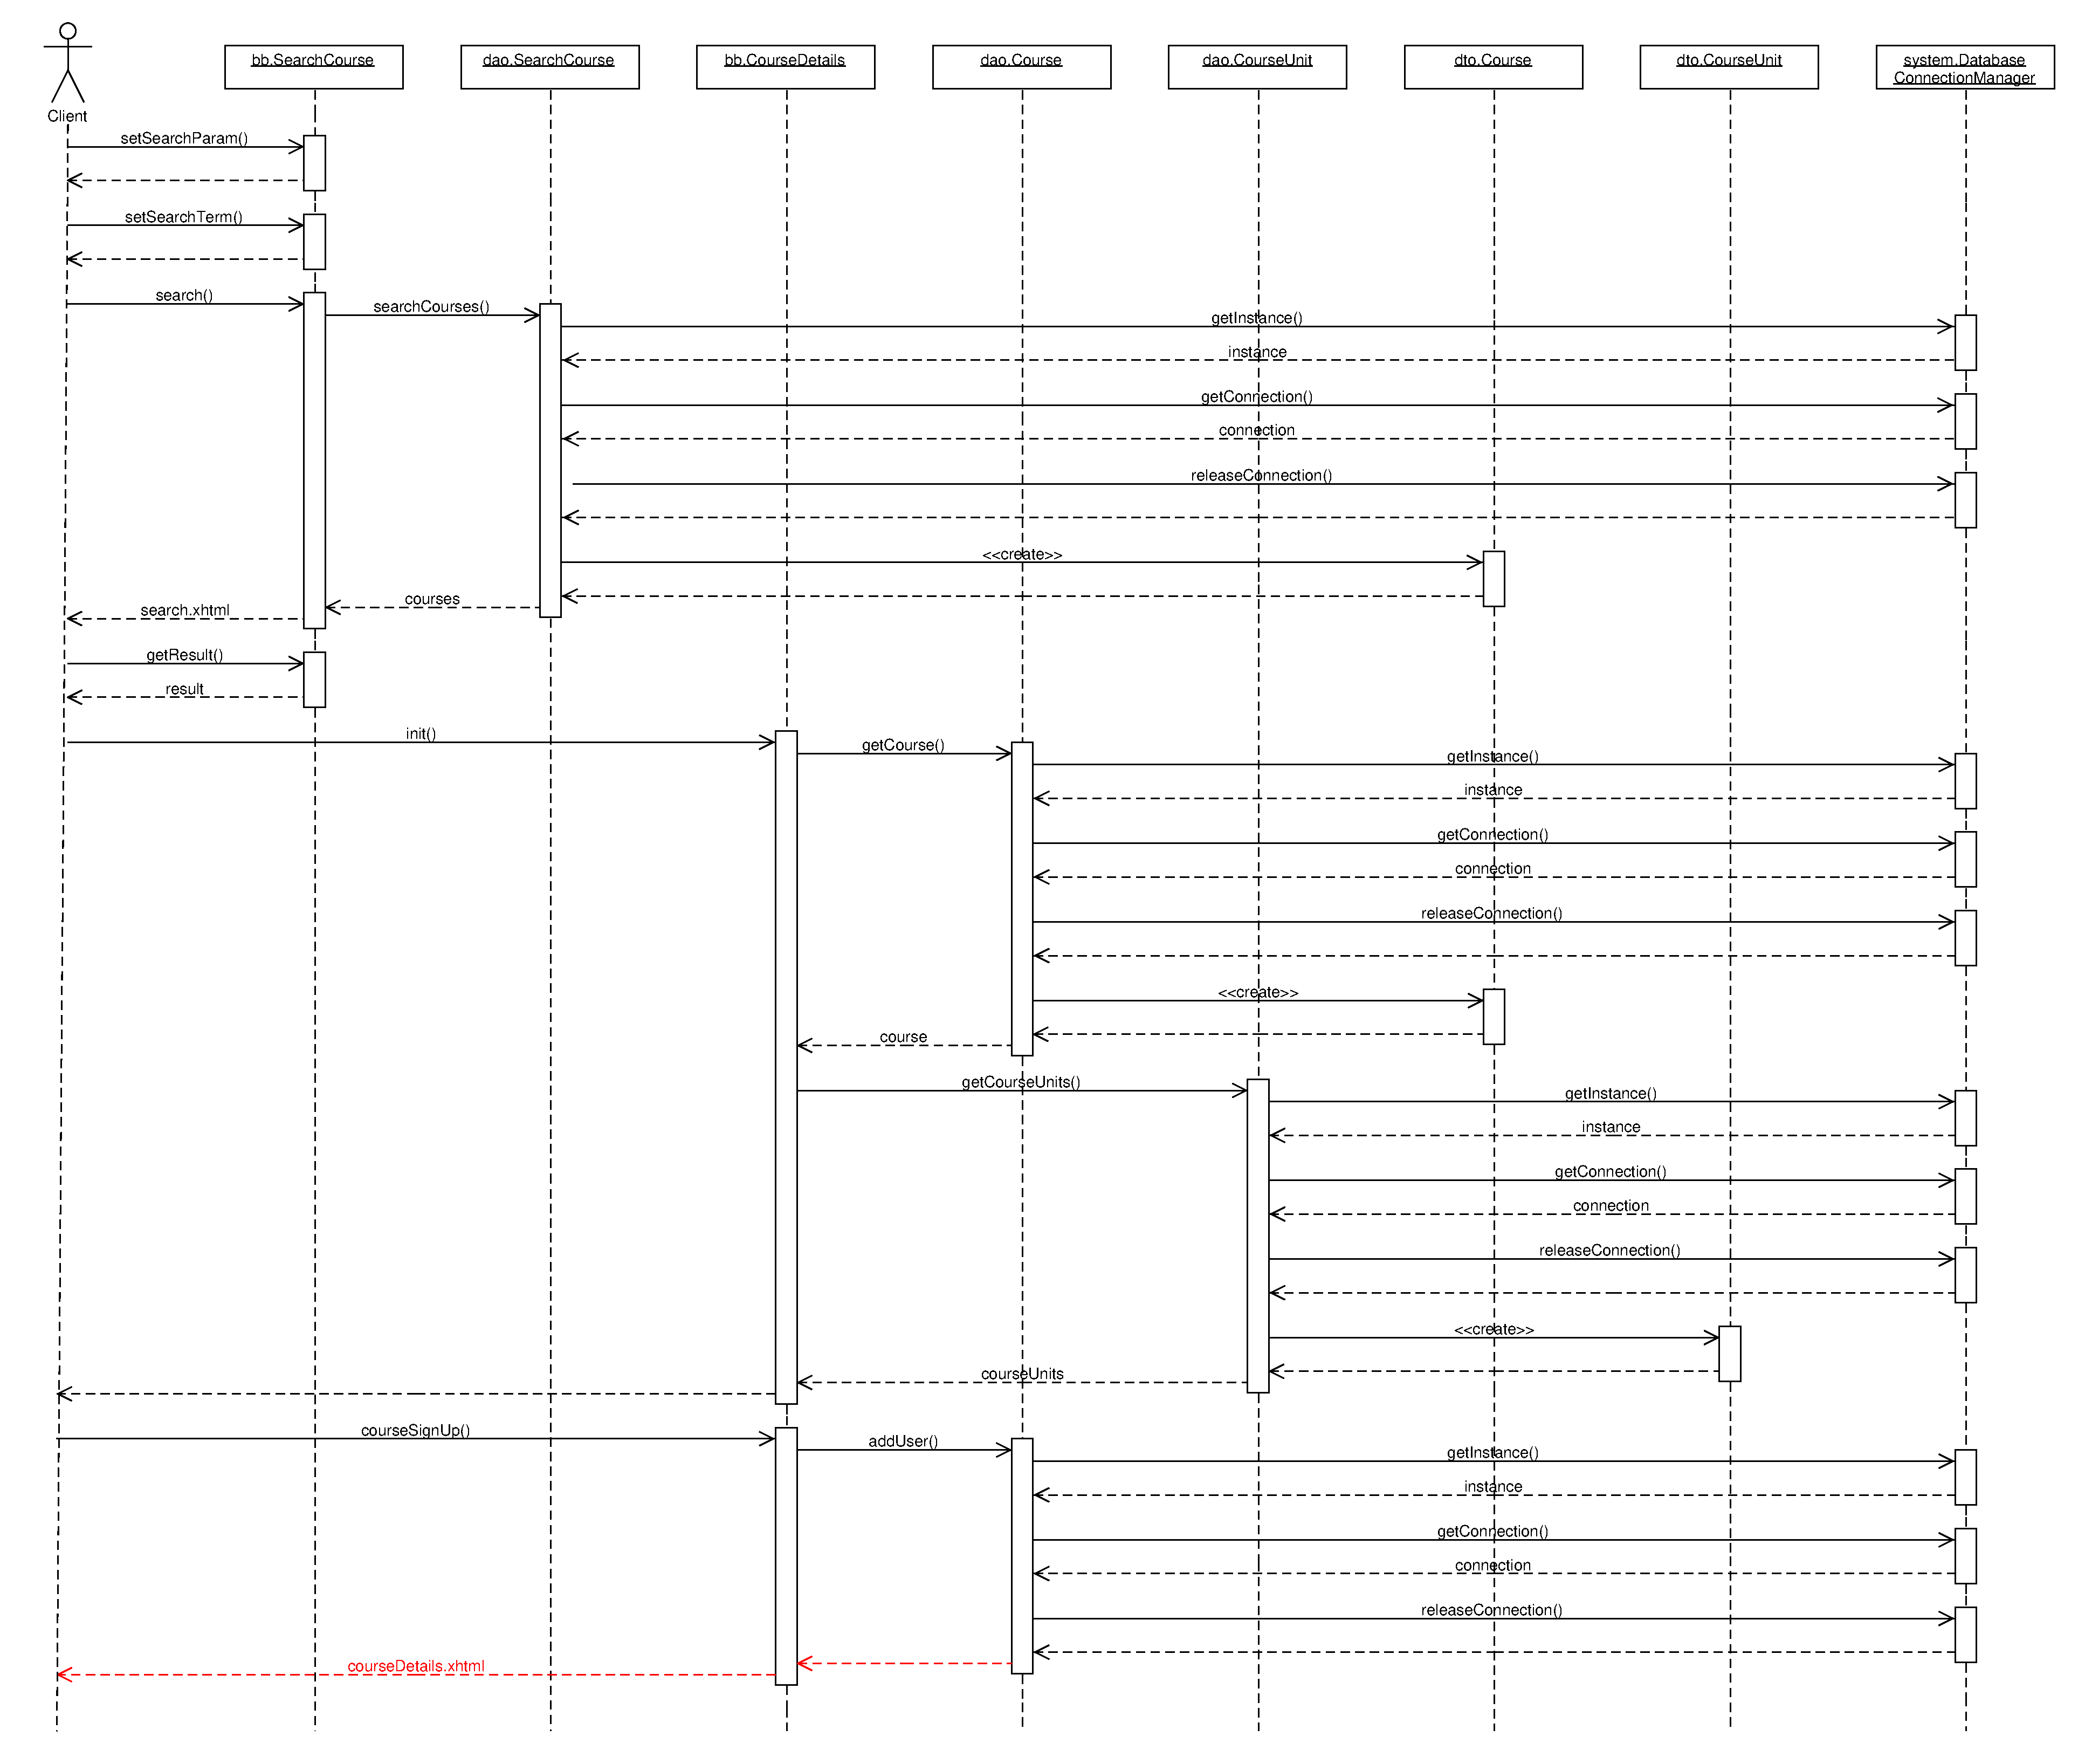
\includegraphics[scale=0.26]{./Grafiken/Sequenzdiagramm-Kursanmeldung.pdf}
\chapter{ER-Modell}

\begin{tiny}
PC
\end{tiny}

\section{Diagramm}

In diesem Kapitel werden die systeminternen Entitäten und deren Relationen untereinander sowie alle dazugehörigen Attribute in einem ER-Diagramm dargestellt und kurz beschrieben.

\includegraphics[scale=0.085]{./Grafiken/ER-Diagramm.pdf}

\section{Beschreibung}
\subsection{User}
Ein im System registrierter Nutzer, welcher entweder als einfacher registrierter Nutzer, oder zusätzlich als Kursleiter, Administrator, oder auch beides gespeichert wird und anhand der 'ID' eindeutig identifizierbar ist. Ein User kann eine Adresse angeben (vgl. 'Address'). Zusätzlich werden die gezahlten Beiträge des Nutzers in der systeminternen Geldstatistik (vgl. 'Statistics') gespeichert, sofern sich dieser zu zahlungspflichtigen Kurseinheiten (vgl. 'Course unit') angemeldet hat. Ein User kann an beliebig vielen Kursen (vgl. 'Course') und Kurseinheiten teilnehmen. Das Attribut 'Course news' beschreibt ob der Nutzer Nachrichten zu einem Kurs abonniert hat zu dem er angemeldet ist. 'E-mail verification' bzw. 'Admin verification' prüfen, ob der Nutzer über seinen persönlichen E-mail Account bzw. durch einen Administrator verifiziert wurde.

\subsection{Course Instructor}
Ein registrierter Nutzer, welcher im System als Kursleiter gespeichert und anhand seiner 'ID' eindeutig identifizierbar ist. Ein 'Course instructor' kann beliebig viele Kurse leiten (vgl. 'Course').

\subsection{System admin}
Ein registrierter Nutzer, welcher im System als Systemadministrator gespeichert ist und anhand seiner 'ID' eindeutig identifizierbar ist. Ein 'System admin' kann sowohl beliebig viele Systemattribute (vgl. 'System attributes') editieren als auch beliebig die Gestaltung der Webanwendung anpassen (vgl. 'Customization data').

\subsection{Address}
Die Anschrift eines registrierten Nutzers bzw. einer Kurseinheit (vgl. 'Course unit'). Diese ist durch ihre 'ID' eindeutig identifizierbar und kann entweder genau einem 'User' oder genau einer 'Course unit' zugeordnet werden.

\subsection{System attributes}
Enthält vom Systemadministrator festgelegte Attribute, welche der Funktionalität der Webanwendung dienen. Diese können bei Bedarf von allen im System gespeicherten Administratoren editiert werden.

\subsection{Customization data}
Enthält den Titel der Webanwendung ('System title'), den Titel der CSS-Datei ('CSS') und kann bei Bedarf von allen im System gespeicherten Administratoren editiert werden.

\subsection{Course}
Ein angebotener Kurs zudem sich beliebig viele Nutzer anmelden können und von mindestens einem 'Course instructor' geleitet wird. Ein 'Course' kann beliebig viele Kurseinheiten (vgl. 'Course units') anbieten und ist anhand der 'ID' eindeutig identifizierbar. Zusätzlich werden die gezahlten Beiträge innerhalb eines Kurses in der systeminternen Geldstatistik (vgl. 'Statistics') gespeichert.

\subsection{Course unit}
Eine Kurseinheit, welche innerhalb genau eines Kurses (vgl. 'Course') angeboten wird und anhand seiner 'ID' eindeutig identifizierbar ist. Sie hat genau eine Anschrift (vgl. 'Address'). An einer Kurseinheit können beliebig viele Nutzer teilnehmen, vorausgesetzt die maximale Teilnehmerzahl ('max. participants') ist noch nicht erreicht. 

\subsection{Statistics}
Die Geldstatistik, welche die über das System eingenommen Geldbeträge ('Amount') an einem bestimmten Datum ('Date') angibt.
\end{document}
